%%% Newden Repository %%%
%%% By: Paulo Vitor Correia de Oliveira %%%
\documentclass[11pt, a4paper]{article}
\usepackage{denplate}

%%% ===== Metadata ===== %%%
\title{Python}
\author{Repositório NewDen}
\date{}

\begin{document}
\maketitle
\void[-3]

\lin
\void[-1]
\tableofcontents
\lin
\newpage

\section{Básicos}

A primeira seção desse capítulo consiste de entendermos como funciona a linguagem de programação Python, vista como uma das linguagens mais simples e rápidas para fazer códigos. Essa versatilidade do Python o torna muito útil para fazer projetos diversos, como jogos, inteligências artificiais, gráficos e dentre outros usos.

\subsection{Tipos Primitivos}

O primeiro conceito que precisamos saber para lidar com uma linguagem de programação é entender como seus dados são guardados. No geral, \textbf{Python trata todos os dados como objetos}, até mesmo os tipos primitivos.

Um objeto é uma \textbf{descrição computacional} de algum tipo de dado. No Python, alguns objetos são ditos como \textbf{tipos primitivos}, isto é, elementos que vão constituir a base de todos os outros. Não significa que todos os objetos são somente os tipos primitivos, mas no geral, todo objeto é uma composição ou extensão deles de algum modo.

No geral, os tipos primitivos do Python são os \textbf{inteiros, }.

\begin{itemize}
    \item \textbf{Inteiro}: O inteiro é a representação de um número pertencente ao conjunto dos inteiros. Considere que a memória é um grande conjunto de bits (um dígito que pode apenas assumir os valores de 0 ou 1) agrupados em grupos de 8 bits, onde cada grupo é o que chamamos de um \textbf{byte}. Cada byte tem um endereço, que é um número Hexadecimal que indica a posição desse byte na memória do computador. Imagine que tenhamos \(B\) bytes de memória e queremos uma forma de representar um número inteiro usando esses bytes disponíveis. 
    
    \(B\) bytes representam \(8B\) bits de memória, portanto, há \(2^{8B}\) valores possíveis para esse conjunto de bits assumir, então, só conseguiremos distinguir no máximo essa mesma quantidade de números. Assim, precisamos decidir quais números vamos representar usando um inteiro com \(B\) bytes. A escolha lógica é preferir os números perto do zero, em um intervalo aproximadamente igual em ambos os lados. Com isso, há várias formas de modelar como usaremos esses bytes.
    
    Uma delas guarda \(1\) bit para representar o sinal do número e os \(8B-1\) seguintes representam o número em sua forma binária, então se \(B=1\), o número \(00010011\) representa o inteiro \(19\) e o número \(10000111\) representaria \(-7\). Nesse esquema, podemos representar todos os números de \([-(2^{B-1}-1),(2^{B-1}-1)]\), onde o zero é representado de duas formas.

    Outra forma seria fazer algo parecido, mas de modo que não perdemos capacidade de representação por existirem duas representações do zero: Representamos os números positivos da mesma forma que antes, usando os últimos \(8B-1\) bits, mas para os números negativos, a representação binária na memória de \(-X\) é o que esperaríamos da representação binária usual do número \(2^{8B}-X\). Essa técnica é chamada de \textbf{complemento de dois}. Novamente, o número \(00010011\) representa o inteiro \(19\), mas o número \(10000111\) agora equivale a \(-121\). Agora, podemos representar todos os números no intervalo \([-(2^{B-1}),(2^{B-1}-1)]\), com o zero possuindo forma única.

    Ainda assim, nenhuma dessas formas é como o Python faz: Ao invés de usarmos um número fixo de bytes para representar um inteiro, o Python faz os inteiros serem definidos dinamicamente, isto é, o objeto do tipo inteiro cresce automaticamente conforme necessário.
    
    Com isso, em Python podemos representar inteiros arbitrariamente grandes, tão grandes quanto sua memória permitir. No geral, é usada a técnica do complemento de dois, porém, se um número em uma variável inteira só precisa de \(B\) bits para ser representado, o complemento de dois é tomado como se estivéssemos usando apenas \(B\) bits.

    \item \textbf{Ponto Flutuante}: Esse é um número mais geral que o inteiro, que nos permite armazenar números reais, porém, com uma representação discreta finita. Chamamos esse tipo de representação de \textbf{ponto flutuante}, que é uma estrutura que muitos computadores usam para lidar com números reais. Nos inteiros, lidamos com a finitude dos bits apenas representando um intervalo contínuo dos inteiros ao redor do zero, que na maioria dos casos, será o intervalo mais relevante. Nos números reais isso não é mais possível: entre quaisquer dois números reais, existem infinitos, então precisamos de outra técnica.

    Há vários padrões distintos de como representar números em ponto flutuante, e por mais que no geral sejam parecidos, vamos usar um padrão, que justamente é o padrão usado no Python: o \href{https://en.wikipedia.org/wiki/IEEE_754}{IEEE 754}. Nesse padrão, representamos um número de ponto flutuante com 8 bytes (ou seja, 64 bits), onde 1 bit representa o sinal do número, 11 bits representam um expoente e os outros 52 representam a mantissa.

    Seja \(e\) o expoente, representando um inteiro de \([-1023,1023],\) onde o número \(X\) é obtido com a representação binária usual de \(X+1023\). Nesse formato, também reservamos o número binário com todos os bits 1 para representar o infinito, usado em alguns contextos.

    Seja também \(m\) a mantissa, representando os dígitos da representação binária do número ignorando a distinção entre parte inteira e decimal. Por fim, também considere como \(s\) o sinal, um bit com valor 1 ou -1.

    Dados esses valores, \textbf{um número X é dado por } \(X=(-1)^s \times (1.m)_{2} \times (2^e)\). Vamos fixar isso com um exemplo.

    Seja \(X=9.875\). O primeiro passo é entender qual a representação de \(X\) na forma binária usual, que é \(9.875 = 2^3+2^0+2^{-1}+2^{-2}+2^{-3} \rightarrow 1001.111\), e agora, fazemos o ponto ir para o local correto: à direita do primeiro um, isto é: \(X=1.001111 \times 2^3\). Com isso, temos que como o número é positivo, o sinal é representado pelo bit 0; A mantissa é dada por \(001111\), que é a parte decimal excluindo o primeiro um e o expoente é 3, representado por \(3+1023=1026=10000000010\). Assim, a representação na memória do número 9.875 é, na forma (sinal + expoente + mantissa):

    \begin{center}
    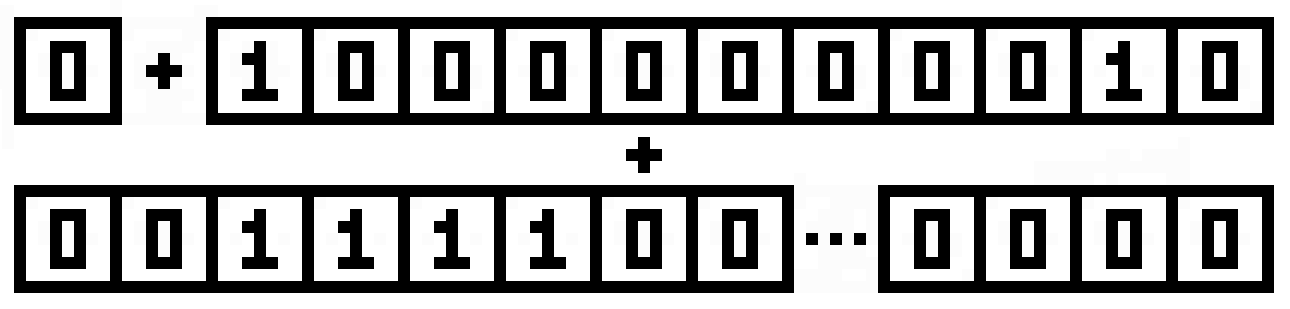
\includegraphics[width=36em]{Imagens/mantissa.png}
    \end{center}

    \item \textbf{Complexo}: O Python também te permite trabalhar com números complexos. Na verdade, é um tipo bem simples: O tipo complexo é basicamente um par de dois pontos flutuantes de tamanho 64 bits, totalizando 128 bits. Um é a parte real, enquanto o outro é o coeficiente da parte imaginária (em Python, a letra \textbf{j} representa a unidade imaginária, e não i). Podemos pegar a parte real e imaginária de um número complexo com .real e .imag, respectivamente.

    \item \textbf{String}: O tipo string é um tipo primitivo que nos permite tratar de textos. Uma string é uma cadeia de caracteres ASCII agrupados com aspas simples ou duplas antes do início e após o fim. Em Python, uma string é imutável, então edições de uma string devem sempre ser feitas criando uma nova string a partir da estrutura de outras.

    Por conta dessa incapacidade de edição de strings, algo a se ficar atento é quando fazer qual operação na string a fim de minimizar sua quantidade de operações para fazer a mesma coisa, já que a imutabilidade torna o código no geral mais difícil de ser implementado de forma eficiente.

    \item \textbf{Booleano}: O tipo booleano é uma variável binária que só pode assumir valores verdadeiro ou falso. Variáveis de outros tipos podem ser interpretadas como booleanos, geralmente associando algo ao falso e todo o resto sendo verdadeiro. Por exemplo, nos inteiros 0 significa falso e todo o resto significa verdadeiro.
    
\end{itemize}

\subsection{Operadores}

    Somente com dados, não podemos fazer muita coisa. Para isso, uma ferramenta que torna possível a manipulação de dados são os \textbf{operadores}. No geral, o Python fornece os operadores aritméticos básicos e alguns adicionais, e por meio deles, podemos criar códigos que façam operações mais complexas. Os principais operadores são:

\begin{itemize}
    \item \textbf{Adição, Subtração e Multiplicação} (\textbf{ + , - , * }): Operadores aritméticos básicos que funcionam como esperado para todos os tipos numéricos. Podem também operar em tipos distintos, onde o tipo mais abrangente prevalece.

    \item \textbf{Concatenação} (\textbf{ + }): O operador de adição pode ser aplicado a strings, onde nesse caso, se torna o operador de concatenação: pega duas strings \(A\) e \(B\) e retorna a junção \(AB\).

    \item \textbf{Divisão e Divisão Inteira} (\textbf{ / , // }): Operador aritmético básico de divisão. O primeiro com uma barra funciona priorizando resultados como ponto flutuante, sendo como uma divisão normal (dentro das limitações do ponto flutuante), enquanto o segundo é uma divisão entre inteiros, que despreza o resto na divisão de um pelo outro e retorna apenas a parte inteira do resultado da divisão.

    \item \textbf{Potenciação} (     \textbf{**} ): Aplica uma potenciação, isto é, eleva um número a algum expoente. Funciona tanto para expoentes inteiros quanto floats.

    \item \textbf{Resto} ( \textbf{\%} ): Operador que retorna o resto de um inteiro na divisão por outro.

    \item \textbf{Atribuição} ( \textbf{=} ): Operador mais usado do Python. Ele é o operador que te permite associar um valor a uma variável, isto é \(A=b \rightarrow\) variável \(A\) tem o valor \(b\).

    \item \textbf{Igualdade e Diferença} (\textbf{ == , != }): Operadores usados para comparar dois valores e retornam um booleano informando se são iguais/diferentes ou não.

    \item \textbf{Desigualdades} ( \textbf{> , < , >= , <=} ): Operadores que comparam números ou outros tipos ordenados, retornando um booleano representando se a comparação é verdadeira. Maior, menor, maior ou igual, menor ou igual.

    \item \textbf{Operadores Lógicos} ( \textbf{ and , not , or , $\wedge$ } ): Fazem comparações lógicas: conjunção, negação, disjunção e ou-exclusivo. Também retorna booleanos operando em booleanos. Uma observação é que o operador ou-exclusivo é denotado matematicamente por \(\oplus\).
    
\end{itemize}

Os operadores possuem uma ordem de precedência para serem aplicados, mas no geral, não é tão necessário saber ela decorada. Ou você usará tanto que se lembrará naturalmente ou você pode usar os operadores de parênteses ( ) para especificar a ordem desejada. Uma outra observação é que podemos separar instruções diferentes tanto por mudar de linha quanto por usar o caractere \textbf{;} e seguir na mesma linha. Veremos agora um código em Python que implementa como poderíamos escrever algumas expressões matemáticas para ficar claro como usamos eles ao escrever o código. (obs: Espaços são opcionais na maioria dos locais)

\textbf{Código 1.2.1: Calcule a expressão \(5^{4-3}+2 \times 6\) e guarde o valor em uma variável \(X\)}

\begin{code}
X = 5 ** (4 - 3) + (2 * 6)
\end{code}

\textbf{Código 1.2.2: Guarde o resto de \(7^{7^{7}}\) na divisão por \(\lfloor105/9\rfloor\) em uma variável \(R\)}

\begin{code}
R = (7 ** (7 ** 7)) % (105 // 9)
\end{code}

\textbf{Código 1.2.3: Guarde em duas variáveis \(M,N\) a maior palavra da língua portuguesa e guarde em uma variável \(O\) o valor da concatenação de \(M\) e \(N\)}

\begin{code}
M = "pneumoultramicroscopicossilicovulcanoconiótico"
N = 'pneumoultramicroscopicossilicovulcanoconiótico'
O = M + N
\end{code}

\textbf{Código 1.2.4: Guarde em uma variável \(Y\) o valor verdadeiro caso uma das condições seja satisfeita: \(R \geq X\), \(X \not\equiv R \text{ (mod 5)} \) e \(\lceil\frac{XR}{1000}\rceil-3>154\)}

\begin{code}
Y = (R >= X) or (X%5 != R%5) or (((X*R+999)//1000) - 3 > 154)
\end{code}

Mas em programação, vale lembrar que nem todo código deve ser executado ao pé da letra simulando na força bruta o que você quer fazer. Ao caminhar lado a lado com a matemática você pode muitas vezes produzir resultados muito mais elegantes e eficientes, visto que o poder computacional não é infinito. 

O seguinte problema é uma forte evidência disso: para Z = 1000, você precisaria executar mais somas que a quantidade de átomos no universo para obter o resultado, mas usando a matemática, podemos obter um resultado para essa expressão facilmente.

\textbf{Código 1.2.5: Dado um inteiro positivo \(Z\), guarde em uma variável \(A\) o valor da expressão abaixo usando uma única linha:}
\[\sum_{k=1}^{2^Z}{\frac{(k\oplus(k-1))+1}{2}}\]

\begin{code}
A = (2**(Z-1))*(Z+2)
\end{code}

\label{c1.2.5}

\textbf{Exercício: Prove que a expressão do problema equivale a \((Z+2)\times2^{Z-1}\). \hyperref[sol_c1.2.5]{Solução}.}

\subsection{Funções}

Assim como na matemática, o Python possui uma forma de definir funções. Funções são trechos de código que recebem uma entrada e retornam uma saída, que executa alguma sequência de operações usando as informações recebidas por essa entrada. A entrada é como se fosse o domínio da função, enquanto a saída é como se fosse a imagem. Além disso, funções em Python podem opcionalmente não retornar valor, não possuir entrada e fazer modificações em trechos externos ao código da função, como outras variáveis.

Um tipo particular de funções são os \textbf{métodos}, isto é, funções já implementadas dentro de um tipo específico que fornecem utilidades comuns de serem exigidas. Python possui no geral uma grande diversidade de métodos. Por exemplo, o tipo string possui muitos métodos interessantes, como o método .replace(P,Q), que te permite substituir as sequências de caracteres que sejam iguais a uma string \(P\) por uma string \(Q\).

Abaixo, seguem alguns exemplos de métodos importantes sendo usados, mas no geral, não precisa decorar todos, apenas estar ciente que existem e quais parecem ser os mais importantes.

\textbf{Código 1.3.1: Use o método replace para apagar as vogais minúsculas da string O.}

\begin{code}
O = O.replace('a','')
O = O.replace('e','')
O = O.replace('i','')
O = O.replace('o','')
O = O.replace('u','')
\end{code}

\textbf{Código 1.3.2: Dados dois números complexos \(C=0.6+0.8j\) e \(D=12-5j\), calcule o módulo do número \(D^{|C|}\).}

\begin{code}
C = .6 + .8j
D = 12 - 5j
modC = (C * C.conjugate()).real ** 0.5
res = D ** modC
modulo = (res * res.conjugate()).real ** 0.5
\end{code}

Métodos são de fato muito relevantes e serão retomados mais em breve. Ainda assim, boa parte das funções não está presa a um tipo específico ou a algum outro objeto, mas sim são em certo sentido globais, seja por sua funcionalidade ou por sua adaptabilidade. Veremos agora algumas funções muito importantes do Python que já vem prontas para você usar e que são muito úteis para diversos fins.

\begin{itemize}
    \item \textbf{Print}: Essa é em muitos locais a primeira coisa que você aprender a fazer em uma linguagem de programação, e de fato faz sentido: essa função nativa do Python nos permite imprimir um texto na tela (ou no terminal). Sua sintaxe é muito simples: print(X) \(\rightarrow\) imprime o valor de \(X\) na tela, onde \(X\) pode ser uma variável, um texto, ou qualquer outra coisa que faça sentido. Também podemos usar um tipo diferente de string que chamamos de \textbf{f-strings}, misturando texto e valores numéricos, nos permitido fazer coisas como frases dinâmicas e também definir quantas casas decimais de um ponto flutuante mostrar ao imprimirmos ele no terminal. A sintaxe de uma f-string é dada por \textbf{f\tb[0.1]"\tb[0.1]texto \{variável\}"}, podendo ter quantas variáveis for necessário.
\end{itemize}

\textbf{Código 1.3.3: Imprima seu nome usando a função print.}

\begin{code}
nome = "Eugênio Costa de Souza"
print(f"{nome}? Sim, sou eu.")
\end{code}

Para definir opções de formatação para a variável, basta adicionar : e depois a especificação que você quer. No caso de casas decimais de um float, basta :.Nf, por exemplo, :.3f, onde N é o número de casas decimais. Você pode usar N como \(\{\text{Variável}\}\) na ocasião do número de casas decimais ser dinâmico.

\textbf{Código 1.3.4: Dado um inteiro \(X\in[0,8]\), imprima o valor de pi com \(X\) casas decimais.}

\begin{code}
X = 5
pi = 3.14159265
print(f"pi = {pi:.{X}f}")
\end{code}

\begin{itemize}
    \item \textbf{Min, Max e Sum}: Funções que retornam o valor mínimo e máximo de um conjunto de números, além da função que retorna a soma dos números. A sintaxe é dada por \(\max(X_1,X_2,...,X_n) \rightarrow X_i\) t.q. \(X_i \geq X_j \tb[0.1] \forall j\). As funções min e sum funcionam de modo análogo, mas retornando o valor respectivo que a função é esperada a retornar.

    \item \textbf{Type Casting}: Por mais que não sejam o que você esperaria de uma função, um local conveniente para se apresentá-las é aqui. Podemos usar algumas funções padrão que nos permitem fazer conversões entre tipos de uma forma que se espera. Por exemplo, podemos converter floats e strings para inteiros, strings para booleanos, dentre outras equivalências razoáveis. Vale lembrar que algumas conversões são feitas implicitamente, por exemplo: ao somarmos inteiros com valores booleanos, eles são convertidos automaticamente, onde valores verdadeiros são 1 e falsos são 0.

\end{itemize}

\textbf{Código 1.3.5: Conversão para inteiro.}

\begin{code}
X1 = 5.13 + 31j
X2 = 36.56
X3 = "20"
X4 = "False"
X5 = ""
print(6 + int(X1.real) + int(bool(X4)) + int(bool(X5)) + int(X3))
\end{code}

Porém, o ponto é que você não precisa ser restrito as funções que o Python te permite usar, na verdade, você pode criar suas próprias funções. A sintaxe disso é:

\begin{code}
def função1(p1, p2, ..., pN):
    <código>
    return resultado
\end{code}

No geral, veja que para definirmos a função usamos a palavra \textbf{def}, seguida pelo nome da função e quais os seus parâmetros. Após isso, usamos : e dentro disso colocamos o bloco de código que representa o que nossa função faz. No final, podemos opcionalmente retornar um valor para quando chamarmos essa função no código. Vamos criar uma função de exemplo para ficar mais claro:

\textbf{Código 1.3.6: Binômio simples}

\begin{code}
qt = 0

def binom(a, b, n):
    global qt
    qt = qt + 1
    return (a + b)**n

print(f'Calculamos os binômios de valores {binom(1,2,3)}, {binom(2,3,5)} e {binom(3,5,8)}, totalizando {qt} binômios.')
\end{code}

Há muitas coisas acontecendo ao mesmo tempo nesse código, então vamos analisá-lo com mais calma. Primeiro, veja que temos uma variável qt inicializada como zero \textbf{fora} da função binom que criamos. Essa função a princípio retorna o binômio \((a+b)^n\), mas veja que ela faz mais duas outras coisas.

A primeira é declarar \textbf{global qt}, e isso basicamente é uma especificação para a função, ela está dizendo que a partir de agora, a variável qt a ser modificada é uma variável global, isto é, fora do escopo da função. Sem essa linha, não podemos editar variáveis externas, visto que o que de fato aconteceria é que uma nova variável qt seria criada do zero quando referenciarmos ela.

Agora, dado que definimos para a função que estamos usando aquela variável externa, podemos modificá-la, e assim, a função incrementa o valor dela em 1 cada vez que é chamada. No fim, quando fazemos o print, veja que chamamos essa função três vezes antes de imprimir o valor de qt, e por isso o valor mostrado é 3, mostrando que qt foi modificada corretamente.

A título de organização, podemos especificar ainda os tipos dos parâmetros e retornos de uma função. Isso é feito usando \textbf{: tipo} para os parâmetros e \textbf{-> tipo} para o retorno, depois do campo dos parâmetros da função.

\textbf{Código 1.3.7: Binômio com tipos explícitos}

\begin{code}
def binom(a:int, b:int, n:int) -> int:
    return (a + b)**n
\end{code}

Por fim, podemos criar funções de uma forma reduzida. Essas são chamadas de \textbf{funções lambda} e apresentam uma sintaxe que começa com a palavra lambda, seguida dos parâmetros separados por vírgula, um caractere : e logo em seguida o valor a ser retornado, tudo na mesma linha. Funções podem ser guardadas em variáveis e chamadas como se o nome da variável fosse o nome delas, e essa característica também está presente nas funções lambda.

\textbf{Código 1.3.8: Binômio reduzido}

\begin{code}
binom = lambda a,b,n: (a+b)**n
\end{code}

\subsection{Condição e Repetição}

Estruturas condicionais são uma parte de extrema importância em qualquer linguagem de programação, pois é a partir delas que tomamos a maioria das decisões diferentes que seu programa deve fazer dada uma entrada ou dado o valor de algo.

A principal estrutura condicional no Python é o comparador \textbf{if}, que possui o seguinte formato:

\begin{code}
if condição_1:
    <código>
elif condição_2:
    <código>
else:
    <código>
\end{code}

Um fato importante para o Python é que todo laço de repetição, estrutura condicional ou qualquer coisa que lide com um bloco de código a frente deve ter indentação correta, por meio de tabs ou espaços. No caso do laço acima, toda vez que entramos dentro do código que deve ocorrer caso a condição seja validada, usamos alguns espaços ou um tab para distinguir isso.

No caso do laço if, a primeira coisa a ser verificada é a condição 1, que pode ser \textbf{qualquer coisa} que seja um valor booleano ou possa ser convertida para um valor booleano, como um inteiro. Caso essa condição seja verdade, então todo o código dentro da seção \textbf{if} será executado, mas os códigos dentro da seção \textbf{elif} e \textbf{else} não serão.

Em caso da condição ser falsa, o código tentará validar a próxima condição: o elif. Se ela for validada, apenas a seção do elif será executada, e caso contrário, ele irá para a próxima seção e seguir o processo. Se chegarmos em uma condição else, significa que independente do que ocorra, chegando aqui o código dessa seção será executado. Assim, em todo bloco condicional \textbf{if} que possua um \textbf{else}, exatamente um bloco de código sempre é executado, dependendo das condições.

Note que foi dito \textbf{que possua um else}, e de fato isso é verdade pois nem todo bloco if precisa de um else ou de elif. No geral, ele sempre deve ter um if inicial, quantos elifs você desejar e opcionalmente pode ou não terminar com um else.

\textbf{Código 1.4.1: Dadas cinco variáveis A,B,C,D,E com valores inteiros distintos, o seguinte código imprime na tela uma palavra com a inicial da maior variável.}

\begin{code}
A = 1; B = -35; C = 0; D = 183; E = -9592
maior = max(A,B,C,D,E)
if maior == A:
    print("Anta")
elif maior == B:
    print("Boto")
elif maior == C:
    print("Canguru")
elif maior == D:
    print("Dromedário")
elif maior == E:
    print("Elefante")
else:
    print("O código foi adulterado!")
\end{code}

Há outras formas de fazermos estruturas condicionais. Em particular, podemos usar o \textbf{operador ternário} que nos permite criar rapidamente um if e um else de uma maneira curta:

\begin{code}
<código> if condição else <código>
\end{code}

Andando de lado a lado com as estruturas condicionais estão as estruturas de repetição. Basicamente, são formas de instruirmos nosso código a repetir certas instruções enquanto alguma condição for válida ou um determinado número de vezes.

Vamos começar com a estrutura mais simples: o laço de repetição \textbf{while}. Sua estrutura é muito simples: Ao chegar na linha do while, ele tem uma certa condição que verificará. Se essa condição retornar um valor verdade, então ele executará o bloco de código dentro dele. Caso for falso, o código para de repetir e segue normalmente para as próximas linhas.

\begin{code}
while condição:
    <código>
\end{code}

Ainda assim, não é a única forma de parar esse laço de repetição: Podemos usar o comando \textbf{break} para forçadamente sair do laço de repetição mais interno que você estiver imediatamente, sem nem mesmo terminar as linhas do bloco que você está executando. Execute o código a seguir e tente descobrir o que acontece. 

\textbf{Código 1.4.2: Sequência misteriosa}
\begin{code}
M = 1; N = 1
while M % 17 != 0:
    M, N = N, M+N-1
    if N % 11 == 0:
        break
    N = N + 1
print(N)
\end{code}

Uma linha que talvez seja confusa seja a terceira, mas saiba que em Python, quando fazemos atribuições de variáveis separadas por vírgula daquela forma, então são múltiplas atribuições feitas respectivamente com a ordem dos elementos dos dois lados.

Além do laço de repetição while, temos um que é usado de uma forma mais comum: o \textbf{for}. Ele possui várias formas básicas de ser usado. Vamos conferir algumas delas.

A principal forma de iteração com for é iterar um número determinado de vezes, e para isso, usamos o objeto padrão do Python chamado \textbf{range}, que nos permite criar um intervalo. Para criar esse objeto, chamamos a função de mesmo nome com os parâmetros necessários. No geral, temos a estrutura:

\begin{code}
for i in range(i0,iN,step):
    <código>
\end{code}

No geral, podemos colocar 1, 2 ou 3 parâmetros na forma usual do range: o início, fim e passo. Se apenas um parâmetro for colocado, ele será o fim. Se dois forem colocados, eles serão início e fim, e se três forem colocados, serão início, fim e passo. Caso o início não seja definido, ele tem valor padrão 0, enquanto o valor padrão do passo é 1. O passo pode ser tanto negativo quanto positivo, e isso impacta o comportamento do range.

O range cria um objeto que contém \(i_0,i_0+step,i_0+2\times step,...,i_0+(k-1)\times step\), onde \(i_0+k\times step\) seria o primeiro valor que alcança ou ultrapassa \(i_N\), no caso, se \(step>0\) então é o primeiro número \(\geq i_N\), e caso \(step < 0\), o primeiro \(\leq i_N\). Vamos fixar com dois exemplos:

\textbf{Código 1.4.3: Encontre quais dos naturais menores que 1000 da forma \(3k+1\) são múltiplos de 11.}

\begin{code}
for i in range(1,1000,3):
    if not i%11:
        print(i)
\end{code}

\textbf{Código 1.4.4: Dado um inteiro positivo \(N\), calcule o valor da torre de potências \(2^{2^{2...}}\) com \(N\) números \(2\).}

\begin{code}
tower = 1; N = 4
for i in range(N):
    tower = 2**tower
print(tower)
\end{code}

\subsection{Complexidade}

Retome ao \hyperref[c1.2.5]{código 1.2.5}. Com o conhecimento que temos agora, conseguimos implementar explicitamente o somatório usando um laço de repetição for. E de fato, o código ficaria o seguinte:

\label{c1.5.1}

\textbf{Código 1.5.1: Retomando um problema anterior}

\begin{code}
Z = 25; sum = 0
for i in range(1,(2**Z)+1):
    sum = sum + ((i^(i-1))+1)//2
\end{code}

Porém, ao tentar executar esse código você vai perceber que mesmo para um valor pequeno com \(Z=25\) o código já começa a ser bem lento. Isso se deve ao número gigantesco de repetições do laço de repetição for: ele cresce exponencialmente conforme \(Z\) aumenta.

Agora suponha que exista um código que para todo valor de \(Z\), resolve nosso problema fazendo exatamente 100 trilhões de operações. Qual dos códigos é melhor: o código 1.5.1 ou esse novo que estamos supondo?

Veja que para valores pequenos de \(Z\), indiscutivelmente o código 1.5.1 é mais rápido: para \(Z \leq 20\), fazemos no máximo alguns milhões de operações para executá-lo, sendo um número muito menor que as 100 trilhões do código alternativo. Porém, com \(Z \geq \log_2(\frac{1}{6}10^{14}) \approx 44\), podemos ver que o nosso código anterior passa a fazer mais de 100 trilhões de operações, e portanto, para qualquer valor de \(Z\) passando disso, a nova versão é mais eficiente.

Assim, o código 1.5.1 só consegue ser mais eficiente para valores pequenos de \(Z\), mas a partir de um certo ponto, ele sempre perderá. Quando isso acontece, dizemos que o código 1.5.1 tem uma \textbf{complexidade maior} que o novo código em função de \(Z\). Um código ser mais complexo que outro significa que conforme o problema aumenta de tamanho, eventualmente esse código sempre ficará mais lento que o outro, onde a diferença entre o número de operações também tende a crescer.

No geral, para problemas escaláveis, queremos que códigos possuam baixa complexidade, pois assim o custo de aumentar o tamanho do problema é o mínimo possível. Por essa razão, uma ferramenta muito importante de computação é fazer análise de complexidade dos códigos. 

Primeiro, vamos definir formalmente uma forma de fazermos isso: Seja \(g(x)\) uma função qualquer e \(op(x)\) a função que calcula quantas operações um determinado código \(K\) faz dada uma entrada de tamanho \(x\). Dizemos que \(K \in O(g(x))\) se \(\exists C \in \Real^{+}, x_0\) onde \(C\times g(x) \geq op(x) \tb[0.5] \forall x \geq x_0\). No geral, \(O(g(x))\) é a classe das funções que são dominadas por um múltiplo de \(g(x)\), então podemos estimar quão rápido o problema vai piorar no pior caso. 

De certa forma, isso nos fornece um limite superior para o código, que é uma boa estimativa para dizer se o tempo necessário para resolver um problema de um certo tamanho é viável. Além disso, não existe só uma classe para limite inferior, também existem um para limite inferior e um para ambos simultaneamente, além de outras classes similares para uma análise mais aprofundada.

\begin{itemize}
    \item \(K \in O(g(x)) \rightarrow \exists C \in \Real^{+}, x_0 \tb[0.5] t.q. \tb[0.5] C\times g(x) \geq op(x) \tb[0.5] \forall x \geq x_0\)
    \item \(K \in \Omega(g(x)) \rightarrow \exists C \in \Real^{+}, x_0 \tb[0.5] t.q. \tb[0.5] C\times g(x) \leq op(x) \tb[0.5] \forall x \geq x_0\)
    \item \(K \in \Theta(g(x)) \rightarrow K\in O(g(x)) \wedge K \in \Omega(g(x))\)
    \item \( \displaystyle K \in o(g(x)) \rightarrow \lim_{x \to \infty}\frac{op(x)}{g(x)}=0\)
    \item \( \displaystyle K \in \omega (g(x)) \rightarrow \lim_{x \to \infty}\frac{op(x)}{g(x)}=\infty\)
\end{itemize}

Com essas funções, podemos calcular a complexidade esperada de trechos de códigos. Vamos ver alguns exemplos.

Primeiro, vamos retornar ao \hyperref[c1.5.1]{código 1.5.1} e calcular sua complexidade. Note que na linha 1, apenas duas atribuições são feitas. Já na linha 2, repetimos \(2^Z\) vezes a linha 3, que faz uma subtração, um xor, uma divisão, duas somas e uma atribuição, totalizando 6 operações. 

Com isso, a grosso modo nosso código faz pelo menos \(6\times 2^Z+2\) operações, fora as operações necessárias para fazer a iteração do for in range. Note que pela definição de complexidade, independente de quantas operações tivessem na linha 3, o código faria algo do tipo \(Q\times 2^Z+2\) operações, e por definição, isso sempre é \(O(2^Z)\). 

Por conta disso, normalmente desprezamos as constantes na hora de calcular a complexidade, apenas analisamos assintoticamente o que está acontecendo, e de cara, vemos que as operações do nosso código crescem linearmente com a função \(2^Z\), mostrando que nosso código é \(O(2^Z)\). 

Por definição, também é verdade que esse código é \(O(3^Z)\), \(O(193^{15Z}+14)\), e dentre outras funções complicadas que assintoticamente crescem mais rápido que \(2^Z\), mas perceba que no geral isso não nos dá muita informação: a melhor informação é obtida sabendo a menor função \(f\) tal que seu código seja \(O(f)\), e no mundo ideal, ele ser \(\Theta(f)\). Ainda assim, algumas vezes pode ser complicado verificar se uma função é \(\Omega(f)\), então na prática em cenários como programação competitiva o que fazemos é estimar a menor ordem de grandeza que garantimos que o código seja \(O(f)\), pois isso normalmente é o suficiente.


\textbf{Código 1.5.2: Dadas duas variáveis \(N\) e \(M\), calcule a complexidade do código.}

\begin{code}
N = 90; M = 50; sum = 0
for A in range(1,N+1):
    for B in range(1,M+1,A):
        sum = sum + 1
print(sum)
\end{code}

No código acima, temos duas variáveis: \(N\) e \(M\) e queremos calcular a complexidade do código conforme elas variam. Como já discutimos, calcular constantes não faz diferença na complexidade final, então vamos prestar atenção na verdadeira parte que gasta operações ali: os dois laços de repetição.

Seu primeiro reflexo pode ser observar que o primeiro vai de \(1\) até \(N\) e o segundo vai de \(1\) até \(M\), então fazemos \(M\) operações \(N\) vezes, sendo isso \(O(NM)\), mas na verdade isso está errado. Considere a seguinte tabela mostrando o valor de sum para algumas combinações de \(N\) e \(M\):

\Table{
 & N=1 & N=5 & N=10 & N=20 & N=50 & N=100 & N=250 & N=500\tl
M=1 & 1 & 5 & 10 & 20 & 50 & 100 & 250 & 500\tl
M=5 & 5 & 13 & 18 & 28 & 58 & 108 & 258 & 508\tl
M=10 & 10 & 24 & 33 & 43 & 73 & 123 & 273 & 523\tl
M=20 & 20 & 46 & 61 & 80 & 110 & 160 & 310 & 560\tl
M=50 & 50 & 115 & 150 & 188 & 251 & 301 & 451 & 701\tl
M=100 & 100 & 229 & 296 & 368 & 474 & 573 & 723 & 973\tl
M=250 & 250 & 572 & 735 & 906 & 1145 & 1340 & 1663 & 1913\tl
M=500 & 500 & 1142 & 1467 & 1806 & 2270 & 2640 & 3179 & 3678\tl
}

Note que se fixarmos \(N=1\) ou \(M=1\), a variável sum parece crescer linearmente nos dois casos, que de fato nos dá a impressão de que ela é linear com \(M\) e \(N\), porém, veja que para outros valores, muitas vezes isso está longe de ser verdade.

Então, vamos tentar calcular corretamente o número de operações. Veja que na iteração \(i\) do primeiro laço de repetição, o segundo laço de repetição será iterado \(\lceil\frac{M}{i}\rceil\) vezes. Assim, ao somarmos todas as \(N\) iterações, temos:

\void[-0.5]

\[\sum_{i=1}^{N}\left\lceil\frac{M}{i}\right\rceil \leq \sum_{i=1}^{N}\left(\frac{M}{i}+1\right)=N+\sum_{i=1}^{N}\frac{M}{i}=N+M\sum_{i=1}^{N}\frac{1}{i}\]

Com isso, perceba que o somatório da direita representa uma área que é estritamente menor que a área em baixo da curva da função \(f(x)=\frac{1}{x}\), como na imagem:

\begin{center}
    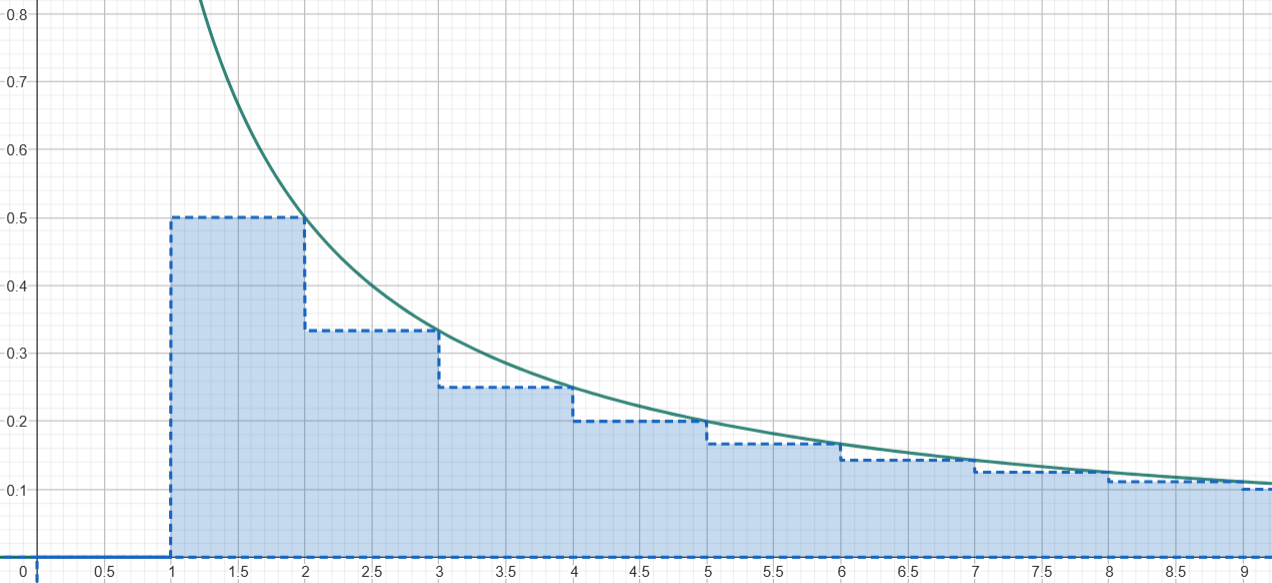
\includegraphics[width=40em]{Imagens/smallharmonicarea.png}
\end{center}

E portanto, podemos estender a desigualdade usando essa área calculando a \href{https://en.wikipedia.org/wiki/Integral}{integral} usando o \href{https://en.wikipedia.org/wiki/Fundamental_theorem_of_calculus}{Teorema Fundamental do Cálculo}:

\[N+M\sum_{i=1}^{N}\frac{1}{i} \leq (N+M)+M\int_{1}^{N}\frac{1}{x}dx=(N+M)+M(\log(N)-\log(1))\]

E assim, temos que a quantidade de operações é limitada por:

\[N+M+M\times\log N=O(N+M\log N)\]

Sendo essa de fato uma boa estimativa para a complexidade do código: podemos comparar os valores dessa função com a tabela e concluir que as estimativas estão muito melhores. 

Um bom exercício é provar que o código também é \(\Omega(N+M \log N)\) e, portanto, \(\Theta(N + MlogN)\). 

\textbf{Exercício: Prove que o código 1.5.2 é \(\Omega(N+M \log N)\). \hyperref[sol_ex1.5.a]{Solução}.}

\label{ex1.5.a}

Por fim, uma observação relevante é que também podemos olhar para a complexidade de espaço dos códigos da mesma forma que olhamos para a complexidade de tempo. Embora não essencial para todos os casos, memória muitas vezes é um recurso caro, principalmente em ambientes corporativos que possuem volumes gigantescos de dados.

\newpage

\section{Estruturas}

Saber lidar com os básicos do Python é de fato essencial, mas não é suficiente para fazer todas as tarefas de forma simples. Um tipo de ferramenta muito útil para isso são as \textbf{estruturas de dados}, que como o nome sugere, são estruturas feitas para armazenar dados de forma eficiente.

\subsection{Estruturas Básicas}

As estruturas mais básicas são extremamente usadas no Python, pois além de simples, tem uma utilidade muito grande. As principais estruturas de dados são \textbf{iteráveis}, isto é, podemos iterar sobre os elementos delas e sem muita dificuldade converter uma na outra com funções específicas do Python. 

Podemos encontrar o tamanho de uma estrutura iterável com a função len(\(estrutura\)), e a partir daqui, definiremos o tamanho atual da estrutura como \(N\). Além disso, as posições da maioria das estruturas iteráveis, assim como do range, tendem a começar com sua posição inicial sendo 0.

\begin{itemize}
    \item \textbf{Lista}: Essa é a estrutura mais simples de todas. Consiste em basicamente um \href{https://en.wikipedia.org/wiki/Array_(data_structure)}{array} de vários valores, independente do tipo, com ordem dos elementos definida e uma enorme variedade de métodos. Uma matriz pode ser representada como uma lista de listas.

    Podemos criar uma lista usando colchetes, cujos elementos estão dentro deles e separados por vírgula: \(lista = [1,\text{'sim'},True]\)

    Entre seus principais métodos, estão:
    \begin{enumerate}
        \item \(.append(x) \rightarrow\) adiciona um elemento \(x\) ao final da lista. Complexidade: \(O(1)\).

        \item \(.insert(i,x) \rightarrow\) adiciona um elemento \(x\) na posição \(i\) lista. Complexidade: \(O(N)\).

        \item \(.remove(x) \rightarrow\) remove a primeira ocorrência de \(x\) da lista. Complexidade: \(O(N)\).

        \item \(.pop(i) \rightarrow\) Remove o elemento da posição \(i\) da lista. Se for chamado sem o parâmetro, remove o último. Complexidade: \(O(1)\) sem parâmetro, \(O(N)\) com parâmetro.

        \item \(.index(x,a,b) \rightarrow\) retorna o índice da primeira ocorrência de \(x\) no intervalo \([a,b[\). Complexidade: \(O(N)\). Quando início e/ou fim não é informado, são usados os valores padrão para início e fim da lista.

        \item \(.sort() \rightarrow\) Caso os elementos da lista possuam uma ordem definida, ordena a lista em ordem crescente. Complexidade: \(O(N \log N)\).

        \item \(.reverse() \rightarrow\) Inverte a lista. Complexidade: \(O(N)\).
    \end{enumerate}

    \item \textbf{Tupla}: Uma versão diferente de uma lista. Armazena uma sequência fixa ordenada e imutável de valores, podendo assim como a lista ser do mesmo tipo ou não.

    Uma tupla pode ser criada usando parênteses: \(tupla = (1,\text{'sim'},True)\)

    Seguem seus principais métodos:
    \begin{enumerate}
        \item \(.index(x,a,b) \rightarrow\) retorna o índice da primeira ocorrência de \(x\) no intervalo \([a,b[\). Complexidade: \(O(N)\). Quando início e/ou fim não é informado, são usados os valores padrão para início e fim da tupla.

        \item \(.count(x) \rightarrow\) retorna o número de ocorrências de \(x\). Complexidade: \(O(N)\).
    \end{enumerate}

    \item \textbf{Conjunto}: Um conjunto é uma coleção \textbf{não ordenada} de elementos únicos de modo que não são guardados por posição, usados para testar pertinência de elementos e eliminar duplicatas. O nome real da estrutura por trás da implementação no Python é \href{https://en.wikipedia.org/wiki/Hash_table}{Hash Table}. 
    
    Podemos criar um conjunto com a função \(set()\) ou com chaves \textbf{necessariamente já preenchidas}: \(\{1,3,11 \}\); \(conjunto = \{1,5,9+3j\}\)

    Entre seus principais métodos, estão:

    \begin{enumerate}
        \item \(.add(x) \rightarrow\) Adiciona o elemento \(x\) ao conjunto caso ele ainda não exista. Complexidade: \(O(1)\).

        \item \(.remove(x) \rightarrow\) Remove o elemento \(x\) caso ele exista, mas gera um erro caso não exista. Complexidade: \(O(1)\).

        \item \(.discard(x) \rightarrow\) Também remove o elemento \(x\) caso ele exista e não gera nenhum erro caso não exista. Complexidade: \(O(1)\).

        \item \(.union([others]) \rightarrow\) Retorna a união de todos os conjuntos. Pode ser chamado com o operador \(|\). Complexidade: \(O(N+len(others))\).

        \item \(.intersection([others]) \rightarrow\) Retorna a interseção de todos os conjuntos. Pode ser chamado com o operador \(\&\). Complexidade: \(O(\min(N,len(others)))\).

        \item \(.difference([others]) \rightarrow\) Retorna a diferença entre esse conjunto e os outros. Pode ser chamado com o operador \(\-\). Complexidade: \(O(N)\).

        \item \(.symetric\_difference([others]) \rightarrow\) Retorna a diferença simétrica dos conjuntos (elementos que só estão em um dos conjuntos). Pode ser chamado com o operador \(\wedge\). Complexidade: \(O(N+len(others))\).
    \end{enumerate}

    \item \textbf{Dicionário}: Estrutura que nos permite criar um mapeamento cujos índices podem não ser posições numéricas, \href{https://discuss.python.org/t/are-dict-class-dictionaries-ordered/38172}{mantendo a ordem de inserção}. Também é implementado internamente com uma Hash Table.
    
    São criados usando a função \(dict()\) ou com chaves vazias ou com os pares já inseridos: \(idades = \{'pedro': 15, 'lucas': 26\}\)

    Dentre seus métodos, temos:
    \begin{enumerate}
        \item \(.get(k,d) \rightarrow\) Retorna o valor com a chave \(k\) ou \(d\) se não existir. Complexidade: \(O(1)\).
        
        \item \(.keys() \rightarrow\) Retorna uma estrutura iterável com as chaves existentes no dicionário. Complexidade: \(O(1)\).

        \item \(.values() \rightarrow\) Retorna uma estrutura iterável com os pares chave-valor existentes no dicionário. Complexidade: \(O(1)\).

        \item \(.items() \rightarrow\) Retorna uma estrutura iterável com os valores existentes no dicionário. Complexidade: \(O(1)\).

        \item \(.update(other) \rightarrow\) Atualiza o dicionário com os dados do dicionário inserido como parâmetro. Complexidade: \(O(len(other))\).

        \item \(.pop(k,d) \rightarrow\) Remove e retorna o valor com a chave \(k\) ou retorna \(d\) se não existir. Complexidade: \(O(1)\).
    \end{enumerate}
\end{itemize}

Uma forma de acessarmos as posições de uma estrutura iterável é com o operador [ ]. Quando em uma lista ou tupla, o argumento dentro dos colchetes deve ser o índice da posição, começando de zero. Se inferidos números negativos, a posição considerada na verdade será do fim para trás, onde \(-i\) pega a posição que em sua frente possuem \(i-1\) elementos. Esse acesso é muito rápido, com complexidade de tempo constante: \(O(1)\).

Um conjunto não guarda elementos por posição, então usamos o operador \textbf{in} para verificar se um elemento pertence a ele, com a sintaxe \textbf{x in conjunto}, que quando está dentro de um if, retorna um booleano que infere se um elemento está no conjunto, com complexidade \(O(\log N)\).

Já em um dicionário, podemos usar também o colchetes normalmente, mas nesse caso, tenha certeza que a chave esteja presente. Caso você não tenha certeza disso, faça isso com o método \(.get()\) ao invés desse operador.

Podemos iterar nessas estruturas usando um \textbf{for x in estrutura}, que itera sobre os valores de uma lista ou tupla, chaves de um dicionário e elementos de um conjunto. Para o dicionário, podemos iterar sobre outras coisas com os métodos \(.keys(), .values(),.items()\).

Algumas vezes queremos algo diferente disso, como iterar simultaneamente sobre os índices e valores de uma lista. Nesse caso, temos a função \textbf{enumerate(e,k)}, que funciona como um range, mas recebe como argumentos um iterável e opcionalmente um valor inicial \textbf{k} e ela cria um iterável de pares \textbf{índice, valor} com base no iterável fornecido. Os índices começam do valor inicial fornecido e aumentam de um em um.

Também existe a função \textbf{zip(e1,e2,...)}, que toma como parâmetros vários enumeráveis e retorna um pareamento deles elemento a elemento. Se vários iteráveis forem fornecidos, são criadas tuplas.

Um método não essencial mas divertido em conjuntos é o \(.pop()\), que remove um elemento do conjunto (o elemento é determinístico, mas depende do Hash), com complexidade \href{https://en.wikipedia.org/wiki/Hash_collision}{média} \(O(1)\).

\textbf{Código 2.1.1: Verificações de Primalidade}

\begin{code}
primos = [2, 3, 5, 7, 11, 13, 17, 19, 23, 29]
pos = {}
conj = set()

primeiro = primos[0]
ultimo = primos[-1]
for i,p in enumerate(primos):
	pos[p] = i
	conj.add(p)
  
for i in range(5):
    conj.pop()

for i in range(primeiro,ultimo+1):
	if i in conj:
		print(f'+1 primo: {i}, na posição {pos[i]} da lista "primos"')
\end{code}

O código acima mostra alguns usos simples do conjunto, lista e dicionário, que são os iteráveis mais usados. Tente interpretar o que cada linha está fazendo.

\subsection{Manipulando Estruturas}

Além de usar métodos e operadores padrão, podemos fazer coisas muito interessantes facilmente usando Python. Uma ferramenta muito legal é o que chamamos de \textbf{compreensão de lista}, uma forma de criar uma lista do zero dada uma função geradora dos elementos:

\begin{code}
lista = [Função for Variável in Iterável]
\end{code}

Vamos fixar isso como um exemplo: Suponha que queremos criar uma lista com os 100 primeiros quadrados perfeitos positivos. É fácil ver que podemos fazer isso como um \textbf{for}, calcular os 100 primeiros quadrados perfeitos e adicioná-los em uma lista, mas uma boa alternativa é comprimir todos esses passos com uma compreensão de lista:

\textbf{Código 2.2.1: Compreensão de Lista}

\begin{code}
quadrados = [x*x for x in range(1,101)]
\end{code}

No geral, segue esse padrão: uma função com variáveis cujos valores possíveis são dados por algum iterável. Podemos inclusive concatenar múltiplos laços de repetição for dentro de uma compreensão de lista, onde o mais a direita será executado completamente a cada iteração do da esquerda.

\textbf{Código 2.2.2: Dado um inteiro \(N\), crie uma matriz \(N\times N\) onde o valor de cada entrada é o produto dos índices da linha e coluna.}

\begin{code}
N = 5
matriz = [[x*y for x in range(N)] for y in range(N)]
\end{code}

Podemos também \textbf{descompactar} estruturas em variáveis, isto é, atribuir elementos respectivamente as variáveis. Há varias formas de fazermos isso: diretamente, com o operador \(*\) para representar múltiplas, com zip, e dentre outras formas. No geral, esteja ciente de que é possível.

\textbf{Código 2.2.3: Descompactando Estruturas}

\begin{code}
lista = [1, 2, 'a', 'b', 1+1j]
tupla = (1, 3, 7, 15)

a,b,c,d,e = lista
x,y,z,w = tupla
p,*meio,q = lista

print(a,b,c,d,e,x,y,z,w,p,meio,q)
\end{code}

Vimos que existe o método \(.sort()\) para ordenar uma lista caso todos os dados possuam uma ordem definida. Por exemplo, se todos eles forem floats ou todos forem strings. Se os dados tem tipos diferentes, não há uma forma lógica de ordenar, então o método não vai funcionar como esperado. Também há uma variação desse método: a função \textbf{sorted()}, cujo parâmetro é uma lista dada e retorna como saída uma cópia ordenada da sua lista:

\begin{code}
    l = sorted([1, 3.6, 5, -3.15, 6])
\end{code}

Além dessas manipulações de estruturas, podemos fazer o que chamamos de \textbf{slicing}: Recortar uma seção contínua da sua lista. Usamos o operador [a:b] para fazer isso, onde \textbf{a} é a primeira posição no slicing e \textbf{b} a primeira posição após o slice. Note que novamente, podemos usar \(-i\) para se referir do final para trás. Ao deixar algum dos lados vazio, também infere-se o valor padrão: 0 para a esquerda e ir até o fim para a direita. 

O slicing não funciona apenas com listas ou estruturas similares, ele também pode ser usados para strings, onde as posições são na verdade os caracteres e o slice retorna uma substring com caracteres da string original. 

\textbf{Código 2.2.4: Exemplos triviais de slicing}

\begin{code}
    l1 = [1,3,5,7,9,11,13,17,21]
    l2 = l1[2:5]
    l3 = l1[5:]

    s1 = "Cavalo Azul"
    s2 = s1[7:]
    s3 = s1[:7]
\end{code}

Com base nessas manipulações, podemos fazer vários tipos de verificações. Por fim, vamos mostrar que é possível utilizar o operador \textbf{else} dentro de um \textbf{for}, onde o trecho else é executado se e somente se não houve break no for.

\textbf{Código 2.2.5: Exemplo de uso de for-else}

\begin{code}
st = "Uma matriz unitária tem colunas ortonormais"
for i,c in enumerate(st):
    if c == 'w':
        print(f'w encontrado na posição {i}')
        break
else:
    print("Frase livre de caracteres w")
\end{code}

\textbf{Código 2.2.6: Dado o código abaixo, encontre o menor valor possível para a variável \(y\) apenas modificando os números de \(x\) de modo que todos eles continuem sendo inteiros positivos distintos. \hyperref[sol_c2.2.6]{Solução}.}

\label{c2.2.6}

\begin{code}
x = [1, 6, 7, 3, 38, 124, 75, 31, 54, 1713]
y = 2**100
for i in range(10):
	if abs(x[i])%5 != 3:
		break
	if abs(x[i])%9 != 4:
		break
	if abs(x[i])%11 != 1:
		break
else:
    y = max(x)
print(y)
\end{code}

\subsection{Pilha e Fila}

Além das estruturas básicas, há muitas outras estruturas frequentemente usadas e que o conhecimento sobre elas se faz necessário para ser um bom programador.

A primeira delas é a \textbf{pilha}, uma estrutura de dados simples que representa a ideia de criar pilhas usando código. Pense por exemplo em uma pilha de livros, quais são as características que descrevem ela? 

Primeiramente, só podemos colocar novos livos no topo da pilha. Também só conseguimos retirar o último livro que foi colocado, pois para remover um livro devemos remover todos os que estão em cima dele. Por fim, conseguimos sempre verificar se a pilha está vazia, e em alguns casos, quantos livros estão na pilha, mas não quais, exceto o do topo.

Essa descrição é factualmente tudo que precisamos assumir para modelar essa estrutura de dados. Em suma, temos que uma pilha é uma estrutura de dados que possui os seguintes métodos:

\begin{itemize}
    \item \(.push(x) \rightarrow\) insere um novo elemento \(x\) na pilha. Complexidade: \(O(1)\).

    \item \(.pop() \rightarrow\) remove o elemento no topo da pilha. Complexidade: \(O(1)\).

    \item \(.top() \rightarrow\) retorna o elemento no topo da pilha. Complexidade: \(O(1)\).

    \item \(.empty() \rightarrow\) retorna um booleano que diz se a pilha está vazia. Complexidade: \(O(1)\).
    
\end{itemize}

Veja que podemos implementar facilmente uma pilha usando a lista sem ter nenhuma perda na complexidade: podemos simular o método push usando \textbf{.append()}, o método pop é equivalente ao pop da lista, o método top pode ser substituído por \([-1]\) e o método empty pode ser obtido usando a função len. 

O mesmo não vale para a \textbf{fila}, que é a estrutura que representa uma fila no mundo real. Diferentemente da pilha, na fila o primeiro a chegar é quem sai, porém, o restante das operações é similar, com o topo da pilha sendo agora a frente da fila. Uma fila possui os métodos a seguir:

\begin{itemize}
    \item \(.push(x) \rightarrow\) insere um novo elemento \(x\) no fim da fila. Complexidade: \(O(1)\).

    \item \(.pop() \rightarrow\) remove o elemento na frente da pilha. Complexidade: \(O(1)\).

    \item \(.front() \rightarrow\) retorna o elemento na frente da fila. Complexidade: \(O(1)\).

    \item \(.empty() \rightarrow\) retorna um booleano que diz se a fila está vazia. Complexidade: \(O(1)\).
    
\end{itemize}

Pelo método pop estar no lado contrário do append, não podemos implementar uma fila usando uma lista tendo a mesma complexidade, já que \(.pop(0)\) é \(O(N)\). Por isso, o natural é usar a estrutura \textbf{deque} da biblioteca nativa do Python \textbf{collections}, capaz de implementar tanto a fila quanto a pilha.

\textbf{Código 2.2.7: Implementando pilha e fila com a biblioteca collections.}

\begin{code}
from collections import deque

pilha = deque(); fila = deque()
pilha.append(1); fila.append(2) #Push
pilha.pop(); fila.popleft() #Pop
pilha[-1]; fila[0] #Top / Front
len(pilha); len(fila) #Empty -> len = 0
\end{code}

Veja que no código acima, há trechos precedidos pelo caractere \#. Em Python, esses são os \textbf{comentários}, que são trechos de código que não impactam seu funcionamento, mas apenas fornecem informação para o programador ler e ter uma compreensão maior de algo. Também há como fazer comentários de múltiplas linhas, onde definimos o início e fim deles com três aspas, simples ou duplas, como em ' ' 'texto' ' ', onde as aspas podem estar em linhas distintas e o texto também.

\subsection{Grafos e Árvores}

Agora vamos ver alguns tipos diferentes de estruturas. Em especial, vamos começar com os \textbf{grafos}. Um grafo é uma estrutura de dados muito popular e muito simples, tendo surgido com o \href{https://en.wikipedia.org/wiki/Seven_Bridges_of_K%C3%B6nigsberg}{problema das sete pontes de K\"{o}nigsberg}, que foi onde o matemático Leonhard Euler descreveu o uso de um grafo pela primeira vez.

Um grafo consiste de um conjunto de vértices \(V\) e um conjunto de arestas \(E\). Vértices são nós que guardam alguma informação, enquanto arestas são como segmentos que servem para conectar os vértices. Há muito para se falar de grafos, mas aqui vamos focar em \textbf{grafos simples não direcionados}: grafos que não podem possuir arestas de um vértice para si mesmo e dados dois vértices \(u,v\), há no máximo uma aresta entre eles, que pode ser usada nas duas direções.

Os valores de um grafo podem ser representados no Python de diversas formas, por exemplo, a forma mais fácil é criar uma lista ou dicionário cuja posição seja o índice de um vértice e o valor na lista seja o valor no vértice. 

Já a estrutura de adjacências é um pouco mais complicada. Temos duas abordagens comumente usadas que vamos citar aqui, que são as mais essenciais para descrever grafos: \textbf{listas de adjacência} e \textbf{matriz de adjacência}.

As \textbf{listas de adjacência} consistem em várias listas de tamanhos variados, uma correspondente a cada vértice que guardam os índices do vértices vizinhos a ele. Assim, podemos percorrer todos os vizinhos de um vértice e verificar se um vértice é vizinho de outro em \(O(\delta(v))\), onde \(\delta(v)\) é o grau do vértice: o número de arestas conectadas ao vértice \(v\). Essa abordagem permite adição fácil de arestas, mas não é tão simples para deletá-las, principalmente quando elas não se encontram na borda da lista (quando outras arestas foram adicionadas depois da que queremos deletar). 

Por outro lado, adicionar e deletar vértices é mais fácil, pois basta descartarmos uma lista e apagarmos no máximo um elemento de cada outra lista, onde implementações com dicionário tornam esse processo consideravelmente rápido. Possui variações que lidam mais rapidamente com situações específicas, como grafos estáticos, de forma mais eficiente. Também possui uma boa versatilidade de espaço, gastando apenas \(O(N+M)\) de espaço, sendo \(N\) o número de vértices e \(M\) o número de arestas, limitado superiormente por \(\frac{N^2-N}{2}\).

Já a \textbf{matriz de adjacência} é uma matriz \(N\times N\) que a posição \(i,j\) guarda se os vértices de índices \(i\) e \(j\) são vizinhos entre si. Essa estrutura dificulta a adição e remoção de vértices, pois implica em remover uma linha e coluna específicas da matriz, que é um processo lento, principalmente se a coluna estiver muito a esquerda. Por outro lado, adicionar e remover arestas é feito muito rapidamente, sempre em complexidade de tempo constante. Um outro ponto negativo é que ela também não é eficiente de espaço: gastando sempre da ordem de \(O(N^2)\) de espaço, pois sempre precisamos criar uma grande matriz.

Para exemplificar esses conceitos, vamos resolver agora o seguinte problema: Dado o grafo abaixo, pinte os vértices de azul ou vermelho de modo que vértices vizinhos não tenham a mesma cor.

\begin{center}
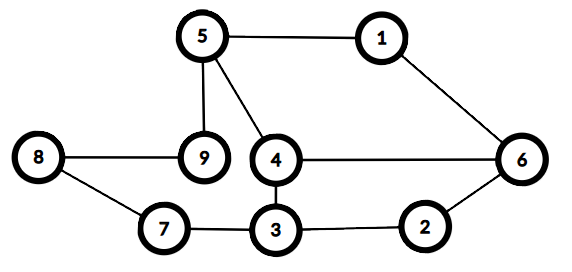
\includegraphics[width=20em]{Imagens/bicolorgraph.png}
\end{center}

\label{ex2.4.a}

\textbf{Exercício: Prove que para todo vértice \(u\) desse grafo, existem pelo menos um vértice \(v\) não vizinho dele de modo que se uma aresta \(uv\) ou for posta, é impossível colorir o grafo com a propriedade citada. \hyperref[sol_ex2.4.a]{Solução}.}

Apesar do exercício acima ser um exercício divertido sobre teoria dos grafos, nosso interesse principal é na representação dele. Assim, vamos mostrar como representamos o grafo e como fazemos um algoritmo que pintará os vértices dessa forma. Primeiro, faremos a versão com listas de adjacência implementadas usando um dicionário de conjuntos:

\textbf{Código 2.4.1: Pintura de grafo bipartido: listas de adjacência}

\begin{code}
from collections import deque

# Versão 1: Grafo com listas de adjacência

adjList = {
    1: {5,6},
    2: {3,6},
    3: {2,4,7},
    4: {3,5,6},
    5: {1,4,9},
    6: {1,2,4},
    7: {3,8},
    8: {7,9},
    9: {5,8}
}

cor = ['','','','','','','','','','']

fila = deque(); fila.append((1,'Vermelho'))
while len(fila) > 0:
    u,c = fila.popleft()
    cor[u] = c
    for v in adjList[u]:
        if not cor[v]:
            fila.append((v, 'Azul' if c == 'Vermelho' else 'Vermelho'))
print(cor[1:10])
\end{code}

Agora, faremos a versão com matriz de adjacência, onde a matriz é representada usando uma lista de listas com números 0 e 1:

\textbf{Código 2.4.2: Pintura de grafo bipartido: matriz de adjacência}

\begin{code}
from collections import deque

# Versão 2: Grafo com matriz de adjacência

adjMatrix = [
    [],
    ['',0,0,0,0,1,1,0,0,0],
    ['',0,0,1,0,0,1,0,0,0],
    ['',0,1,0,1,0,0,1,0,0],
    ['',0,0,1,0,1,1,0,0,0],
    ['',1,0,0,1,0,0,0,0,1],
    ['',1,1,0,1,0,0,0,0,0],
    ['',0,0,1,0,0,0,0,1,0],
    ['',0,0,0,0,0,0,1,0,1],
    ['',0,0,0,0,1,0,0,1,0]
]

cor = ['','','','','','','','','','']

fila = deque(); fila.append((1,'Vermelho'))
while len(fila) > 0:
    u,c = fila.popleft()
    cor[u] = c
    for v in range(1,10):
        if adjMatrix[u][v] and not cor[v]:
            fila.append((v, 'Azul' if c == 'Vermelho' else 'Vermelho'))
print(cor[1:10])
\end{code}

Novamente, não provaremos aqui que algoritmo funciona, mas se tiver interesse, confira os comentários na solução do exercício citado. Dito isso, veja que nessa situação, há várias observações que podemos fazer. Primeiro, no código 2.4.1 poderíamos otimizar o tempo de criação das listas de adjacência substituindo o dicionário de conjuntos por uma lista de listas também, já que nesse caso, nosso grafo é fixo. 

Além disso, veja que fazendo isso, o tempo e espaço da solução com matriz de adjacência é visivelmente maior que o da lista de adjacência, pois tanto criamos posições desnecessárias na matriz quanto acessamos posições desnecessárias e ainda fazemos mais comparações. Em outros cenários, como \textbf{queries} de arestas ou vértices, poderíamos comparar como é o desempenho de cada método, mas a partir do momento que se sabe fazer a análise assintótica das complexidades e também a ideia chave da implementação, isso se torna um detalhe relativamente simples que você terá contato eventualmente.

Agora, veremos uma classe especial de grafos: as \textbf{árvores}, que são definidas como grafos acíclicos conexos. Um grafo acíclico é um grafo que não tem ciclos: uma sequência de vértices distintos ligados por arestas que eventualmente volta para o vértice inicial. Já um grafo ser conexo significa que para todo par de vértices, existe uma forma de chegar de um até o outro percorrendo arestas.

Essa definição pode parecer sem importância, mas ela te dá \href{https://en.wikipedia.org/wiki/Tree_(abstract_data_type)}{uma enorme quantidade de propriedades de brinde}. No geral, uma árvore tem \(N\) vértices, \(N-1\) arestas, possui caminho único entre qualquer par de vértices, e possui uma representação muito eficiente.

\begin{center}
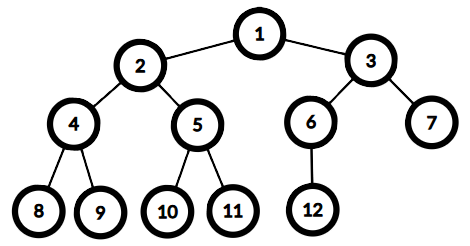
\includegraphics[width=20em]{Imagens/binarytree.png}
\end{center}

A imagem acima representa uma árvore. Ao fixarmos um vértice e chamá-lo de \textbf{raiz}, podemos organizar a árvore nessa estrutura onde os vizinhos sempre estão uma camada abaixo, e chamamos isso de \textbf{nível} de um vértice em relação a essa raiz. Quando uma árvore enraizada possui no máximo dois filhos, ela é chamada de \href{https://en.wikipedia.org/wiki/Binary_tree}{árvore binária}. Em uma árvore, folhas são os vértices das pontas de uma árvore: nesse caso, 7,8,9,10,11 e 12. Além disso, uma árvore binária é balanceada se a diferença máxima entre o nível de duas folhas é no máximo 1.

Todas essas definições são naturais e muito frequentes quando trabalhamos com árvores, então por mais que seja um pouco chato receber chuvas de definições assim do nada, é um requerimento para termos um conhecimento melhor sobre elas.

Como uma árvore é um grafo, podemos representar ela da mesma forma que um grafo. Apesar disso, e tivermos uma raiz fixada, podemos representar uma árvore de outra forma: basta representar as arestas por um vetor que mostra quem é o vértice pai de cada vértice. Para muitos problemas, essa é uma forma muito mais simples e útil de representar:

\label{c2.4.3}
\textbf{Código 2.4.3: Dada a árvore representada na figura logo acima, crie uma função que dado um vértice \(u\), retorne a quantidade de arestas no caminho de \(u\) até a raiz.}

\begin{code}
pai = [0,0,1,1,2,2,3,3,4,4,5,5,6]

def distancia(u):
    dist = 0
    while pai[u]:
        dist = dist + 1
        u = pai[u]
    return dist
\end{code}

Se quisermos usar a função várias vezes, essa solução não é a mais eficiente de todas, mais ainda assim é extremamente simples se compararmos com o que precisaríamos escrever para representar como um grafo qualquer. Quando falarmos de programação funcional, exploraremos mais conceitos interessantes envolvendo árvores, mas de início, tenha ciência do que é uma árvore e de suas principais propriedades.

\subsection{Heap}

Há mais uma estrutura muito importante e um pouco mais complexa a tratarmos aqui: a \textbf{heap}, também chamada de \textbf{fila de prioridade}.

Seu nome vem do fato que ela representa algo similar a uma fila, mas os elementos tem um certo "valor de prioridade", onde o termo com maior mais extremo sairá primeiro ao usar o método pop. No geral, existem dois tipos de fila de prioridade: a \textbf{max heap} e a \textbf{min heap}. Definiremos aqui a max heap, mas basta inverter os locais em que aparece o máximo por mínimo. Em particular, uma max heap em que você guarda o valor \(x\) como \(-x\) se comporta como uma min heap. Uma max heap possui os seguintes métodos:

\begin{itemize}
    \item \(.push(x) \rightarrow\) insere um novo elemento \(x\) na heap. Complexidade: \(O(\log N)\).

    \item \(.pop() \rightarrow\) remove o elemento máximo da heap. Complexidade: \(O(\log N)\).

    \item \(.top() \rightarrow\) retorna o elemento máximo da heap. Complexidade: \(O(1)\).

    \item \(.empty() \rightarrow\) retorna um booleano que diz se a heap está vazia. Complexidade: \(O(1)\).
    
\end{itemize}

Como você pode ver, no geral as operações parecem muito parecidas com a de uma pilha ou fila normal, mas há duas diferenças principais: ela lida com elementos máximos, e isso não é mais tão intuitivo de fazermos. Além disso, a complexidade do seus métodos push e pop agora são \(O(\log N)\), que não é mais intuitivo o que fazer para conseguirmos fazer isso se fossemos implementar.

A resposta para esses mistérios é que por baixo dos panos, a heap tem o formato de uma árvore: os elementos em uma heap são guardados de uma forma que a posição \(x\) é filha da posição \(\lfloor \frac{x}{2}\rfloor\) e o pai sempre é maior ou igual ao filho (o contrario na min heap).

Com base nisso, podemos pensar em uma função de push e pop que mantenha essa propriedade, e assim, podemos sempre garantir que o elemento máximo é a raiz da árvore. Mostraremos como fazer isso.

Primeiramente, perceba que ainda não vimos como se implementam métodos. Por isso, faremos os métodos da heap de uma forma um pouco diferente: faremos funções push, pop, top e empty que tomam um argumento \(h\), que representa a lista com os valores da heap, e após isso, o restante dos argumentos (se houver). A princípio, isso não muda muito a dinâmica da situação, já que se tivermos uma heap \(h\), chamaremos o método com \textbf{método(h,parâmetros)} ao invés de \textbf{h.método(parâmetros)}.

\textbf{Código 2.5.1: Métodos empty e top de uma heap}

\begin{code}
heap = ['max']

def empty(h:list):
    return len(h) == 1

def top(h:list):
    return h[1] if not empty(h) else None
\end{code}

Esse é o começo do nosso código da heap, e já há algumas coisas para se comentar dele. Primeiro, veja que a heap como definimos induz a pensarmos que a raiz da árvore é o vértice de valor 1, assim como na figura que vimos há alguns momentos atrás. Ainda assim, uma lista sempre começa com o índice zero. O que fazemos com a posição zero, já que não a usaremos na heap?

Na verdade, tem várias formas de você lidar com isso. Uma delas é você abstrair o número de posição, e fazer a posição conceitual \(i\) ser guardada na posição \(i-1\) da lista, assim, a raiz de fato poderia ser guardada no zero sem problemas. Em particular, eu não gosto muito dessa solução, pois tende a deixar o código desnecessariamente mais confuso.

Uma outra possível solução seria utilizar a posição zero para guardar alguma informação adicional, e nesse caso, usar as outras posições normalmente sem tocar na posição zero. Essa será a maneira que trabalharemos: guardaremos o tipo da heap a posição zero, \textbf{max} para uma max heap e \textbf{min} para uma min heap. Em particular, implementaremos a max heap.

Ainda assim, esse método não é perfeito: perdemos agora a capacidade de obter o significado ideal da função len quando aplicada a lista da heap, pois agora ela retorna o sucessor do número de elementos pela existência do elemento extra. Detalhes assim podem ser resolvido com \textbf{orientação a objetos}, que é um tema que vamos explorar mais a frente no documento. Por enquanto, apenas aceite essa modelagem.

Dito isso, é fácil ver que as funções propostas agora cumprem o significado esperado: empty diz se há algum elemento fora o elemento extra e top retorna o primeiro elemento que não seja o extra, e no caso de estar vazia, retorna o valor \textbf{None}. Esse valor nada mais é que um tipo especial para representar ausência de valor que existe em Python. Por padrão, você poderia fazer seu comportamento retornar outra coisa, como um zero, -1 ou outro número significativo, mas escolhas assim variam conforme seu uso e não faz tanta diferença, contanto que você documente o que você decidiu fazer.

Agora, vamos começar a parte divertida: Fazer a função \textbf{push}. A princípio, vamos partir do pressuposto que nossa heap tem o formato esperado: \(x\) é filho de \(\lfloor \frac{x}{2} \rfloor\) e o pai é maior ou igual ao filho. No nosso caso base: a heap está vazia, usar o método append é suficiente para executar o push com sucesso, mas em um caso arbitrário, não necessariamente: falta assegurar que essa posição adicionada é de fato menor ou igual a seu vértice pai.

Note que por definição, a única relação potencialmente errada é a do nosso novo vértice \(x\) com seu pai, então a primeira coisa que vamos fazer é: se o vértice \(x\) for maior que o vértice \(\lfloor \frac{x}{2} \rfloor\), então trocamos eles de lugar.

Agora, essa relação está correta, mas será que todas as outras continuam corretas? Bom, veja que como o vértice \(\lfloor \frac{x}{2} \rfloor\) é menor que \(x\), então trocá-los de lugar certamente não estraga a relação com o outro filho de \(\lfloor \frac{x}{2} \rfloor\), pois o valor do pai dele só aumentou. Por outro lado, isso pode sim estragar a relação com o pai de \(\lfloor \frac{x}{2} \rfloor\), pois agora o seu filho pode ter ultrapassado seu pai.

No geral, corrigimos o problema entre \(x_1=\lfloor \frac{x}{2} \rfloor\) e \(x\), mas agora temos um problema entre \(x\) (que ocupa a posição de \(x_1\)) e \(x_2=\lfloor \frac{1}{2}\lfloor \frac{x}{2} \rfloor\rfloor\). 

Agora, o que fazemos é repetir o processo: se for necessário trocar \(x\) e \(x_2\) de lugar, note que os filhos de \(x\) nem de \(x_2\) terão problemas: os filhos de \(x\) agora serão filhos de \(x_2\) que é maior que o antigo pai deles \(x_1\), e os filhos de \(x_2\) agora serão filhos de \(x\) que também é maior que o antigo pai deles \(x_2\). Com isso, novamente a única relação que pode ter problema é \(x\) (na posição de \(x_2\)) com o pai de \(x_2\). 

Perceba que ao repetirmos esse processo até chegar na raiz, toda a árvore não terá mais problemas, pois a raiz não possui um pai para gerar conflitos, e então, conseguimos corrigir a árvore. A complexidade desse processo é \(O(\log N)\) pois uma árvore com \(N\) nós possui altura \(\lfloor\log_2(N)\rfloor+1\), sendo essa a constante de proporcionalidade de quantas vezes repetimos o processo de passos constantes.

Agora, vamos ver como fica o código que descreve esse procedimento usando Python: Usaremos uma variável auxiliar \textbf{nx} que representa o índice do vértice que possivelmente tem problema com seu pai no dado momento e repetiremos até acabar.

\textbf{Código 2.5.2: Método push de uma heap}

\begin{code}
def push(h: list, x):
    nx = len(h)
    h.append(x)
    while(nx > 1):
        if h[nx] > h[nx//2]:
            h[nx],h[nx//2] = h[nx//2],h[nx]
            nx //= 2
        else:
            break
\end{code}

Um primeiro detalhe de notação é que existe a linha \textbf{nx //= 2}, que pode ser estranha. Isso se chama atribuição, que é quando colocamos um operador de igual na frente de um operador, e ele fará o mesmo que \(x (f=) y \leftrightarrow x = x f y\), ou seja, fará a operação e substituirá o valor da variável \(x\) pelo novo valor da variável \(xfy\), dado o argumento \(y\). A partir daqui usaremos as notações alternadamente, mas é apenas uma das curiosidades úteis que você deve aprender pelo caminho.

Veja que descrevemos exatamente o que dissemos: troca o pai e filho caso a relação entre eles esteja errada e diz que a próxima posição candidata a estar errada é a do pai.

Um detalhe é que estamos executando enquanto \(nx>1\) pois a igualdade infere que chegamos na raiz, que temos certeza que não tem problemas com o pai. Já o break na condição else é uma otimização pois se sabemos que o único par que poderia ter problemas não tem, então a heap está totalmente bem estruturada.

Agora, vamos verificar o método pop. No geral, queremos retirar e retornar o maior elemento, que sabemos com certeza que é a primeira posição. Porém, note que não é tão simples quanto apenas apagar e retornar: queremos fazer essa operação em tempo logarítmico, mas usar diretamente o método pop da lista para a primeira posição teria tempo linear, e além disso, a lista resultante não manteria o formato da heap com as propriedades necessárias.

Para fazermos rapidamente a operação de remoção, o truque é trocar a primeira e a última posição de lugar, remover a última posição que agora tem o maior valor e tentar corrigir a árvore a partir disso.

Primeiro, vamos corrigir a maior posição: sabemos que com certeza ela é um dos filhos da maior posição pela estrutura anterior da árvore, então, basta trocar com o lado que for maior e corrigiremos o maior elemento. Por consequência, o outro lado da árvore já está correto: ele só tinha o maior elemento como problema, mas agora não tem mais. Então, basta corrigir para o lado que o elemento pequeno foi.

Perceba que isso segue a mesma estrutura do método push: As únicas relações que tinham problema eram do vértice \(x=1\) com seus filhos, e agora são de um dos seus filhos com os filhos dele. Pela mesma lógica, conseguimos repetir esse processo até chegar nas folhas e corrigir a árvore toda, sendo com complexidade \(O(\log N)\) pelo mesmo argumento, somado ao fato que o pop na última posição custa \(O(1)\).

Com isso, faremos algo parecido para construir o código, mas com algumas sutilezas: na implementação, no final temos que retornar o último elemento de \(h\), visto que ele é quem agora contém o valor de quem era o primeiro elemento. 

Além disso, temos que lembrar de escolher o filho da esquerda sempre que ele for maior \textbf{ou} não existir filho da direita, pois se não olharmos para essa situação, ele estará fazendo o filho da direita ser comparado com a posição que apenas guarda o maior elemento, que quase sempre irá ser trocada por ser o maior elemento e assim estragando nosso algoritmo, visto que essa posição teoricamente não existe mais.

\textbf{Código 2.5.3: Método pop de uma heap}

\begin{code}
def pop(h: list):
    if empty(h):
        return None
    nx = 1
    h[1], h[len(h)-1] = h[len(h)-1], h[1]
    while 2*nx <= len(h)-2:
        x = 0
        if 2*nx+1 > len(h)-2 or h[2*nx+1] < h[2*nx]:
            x = 2*nx
        else:
            x = 2*nx + 1
        if h[nx] < h[x]:
            h[x],h[nx] = h[nx],h[x]
            nx = x
        else:
            break
    return h.pop()
\end{code}

Esse código é consideravelmente mais complicado, mas veja que ele faz exatamente o que estamos falando: primeiro troca a primeira com a última posição (sendo justamente a posição que ele retorna no final, usando \textbf{return h.pop()}).

Durante a execução do while, nossa condição é justamente o filho de menor valor ser no máximo len(h)-2, que é exatamente o maior índice da heap depois que removermos o último. Da mesma forma, logo abaixo definimos qual o maior filho, se atentando ao detalhe de quando o filho da direita não existe. Por fim, executamos a troca quando necessário e quando não, encerramos, assim como no método push.

Agora, você pode se divertir testando e entendendo esse código mais profundamente, verificando que ele realmente faz o que se propõe.
\newpage

\section{Paradigmas}

Paradigmas são estilos de programar: adotar alguns princípios e construir seu código com eles em mente. Nessa seção, veremos dois paradigmas muito importantes em Python, a \textbf{programação funcional} e \textbf{programação orientada a objetos}.

\subsection{Explorando Funções}

    O primeiro paradigma que veremos é a programação funcional, mas antes de vê-lo, é necessário que exploremos um pouco mais as funções para ter uma noção mais profunda de seu potencial e entender a razão que esse paradigma é importante.

    Vamos começar com algo muito comum que até o momento foi secretamente evitado em várias partes desse documento, mas que quem já possui esse conhecimento provavelmente percebeu: o uso de \textbf{recursividade.}

    Uma coisa muito boa de funções é que ela funciona muito bem se a usarmos de uma forma similar a como usamos a indução: muitas vezes conseguimos facilmente resolver uma iteração da função para um caso maior se assumirmos que nossa função funciona corretamente para casos menores e prestar atenção aos casos base.

    No geral, recursão consiste em chamar a função dentro dela mesma e com base no resultado dessas chamadas internas, resolver a chamada anterior. Vamos ver um exemplo para entender melhor como isso funciona.

    Retome o \hyperref[c2.4.3]{código 2.4.3}. O seu objetivo é criar uma função que retorna a quantidade de aresta do caminho até a raiz. Vamos refazer esse código usando recursividade e explicar o que fizemos.

\textbf{Código 3.1.1: Caminho até a raiz novamente.}

\begin{code}
pai = [0,0,1,1,2,2,3,3,4,4,5,5,6]

def distancia(u):
    if not pai[u]:
        return 0
    return distancia(pai[u]) + 1
\end{code}

Veja que aquele já era um código simples, mas esse está absurdamente simples, mas veja que a ideia dele é totalmente intuitiva. Qual seria o caso base de um problema de distância até a raiz? Bom, é fácil perceber que é justamente a raiz, que tem distancia zero. Assim, nossas primeiras duas linhas da função apenas verificam se estamos no caso base e se estivermos, retorna que a distância é zero.

Agora, faltam todos os outros casos, mas perceba o seguinte, dado que a nossa árvore está enraizada, então o caminho até a raiz é dado subindo vértices. Assim, se não estamos no caso base, basta ver quantas vezes teríamos que subir se estivéssemos no pai desse nó e somar 1, pois precisamos subir até ele.

Vamos agora ver outro exemplo, só para deixar claro como conseguimos usar recursão para simplificar problemas de uma forma muito grande usando códigos extremamente simples em relação com a iteração tradicional.

O algoritmo de Euclides é um algoritmo matemático muito famoso e uma forma muito simples de encontrar o máximo divisor comum de um número. Ele é descrito da seguinte forma: Sejam \(a,b\) dois valores que queremos encontrar o maior divisor comum.
\begin{itemize}
    \item Se um dos números for zero, por definição, o outro número é o maior divisor comum dos dois números, visto que zero é múltiplo de tudo.

    \item Caso contrário, suponha sem perda de generalidade que \(a<b\). Então, o \(mdc(a,b)\) é um número \(k\) tal que \(a=ka_1, b = kb_1\). Com isso, faça \(c=b-a=k(b_1-a_1)\). O \(mdc(a,b)\) é o mesmo que \(mdc(c,a)\), então, faça o processo com esses novos números, que são menores, até um deles ser zero e acharmos o valor de \(k\).
\end{itemize}

Lendo uma descrição assim, parece que há vários passos para fazer: verificar se \(a\) é zero e retornar \(b\), verificar se \(b\) é zero e retornar \(a\), verificar qual dos dois é o maior para fazer a subtração, de fato fazer a subtração e pensar em uma forma de iterar sobre isso com um código eficiente. Com recursão, podemos explorar as propriedades do \(mdc\) e fazer \textbf{\textit{o maior código de todos os tempos}} para calcular o \(mdc\):

\textbf{Código 3.1.2: Código que calcula o máximo divisor comum.}

\begin{code}
def mdc(a,b):
    if a == 0:
        return b
    return mdc(b%a, a)
\end{code}

Agora, vamos ver para onde foram todos os problemas: Note que se \(a > b\),  a próxima chamada da função será \(mdc(a,b)\), e então o código prosseguirá corretamente. Caso contrário, ele recebe \(a<b\) e mantém \(a<b\).

Por essa mesma razão, só precisamos verificar se \(a\) é zero, pois se \(b\) for, ele será detectado na próxima chamada da função. 

Por fim, veja que subtrações sucessivas do menor número no maior número equivale a fazermos o operador resto na divisão de \(b\) sobre \(a\), pulando ainda vários passos de uma vez, embora o código também funcione se usarmos apenas a subtração.

Funções também podem receber números arbitrários de parâmetros quando não sabemos o que queremos fazer. Podemos implementar isso escrevendo o \textbf{operador de descompactamento} * antes do parâmetro, indicando que uma quantidade variável de parâmetros caberá ali, onde a função então agrupará eles em uma tupla. 

Note que podemos ter sim outros parâmetros nos argumentos da função, mas devemos ou colocar eles no início para a função entender que todos que sobrarem são os múltiplos, ou devemos especificar os parâmetros com \textbf{nome do parâmetro = valor}.

Além disso, podemos também usar ** antes do argumento, mostrando que receberemos argumentos nomeados que serão capturados usando um dicionário, e nesse caso, passar o parâmetro \textbf{filha='Ana'} te permite obter tanto o nome filha quanto nome o 'Ana' dentro da função, nos possibilitando a usarmos como for necessário.

Vamos fazer um grande exemplo para fixar bem esses conceitos. Se necessário, brinque um pouco com esse código, modifique as funções e faça suas próprias ideias funcionarem.

\label{c3.1.3}
\textbf{Código 3.1.3: Miscelânea de funções multiparâmetros.}

\begin{code}
def mdc(a,b):
    if a == 0:
        return b
    return mdc(b%a,a)

def soma(a,b):
    return a+b

def apply(*nums,func,x0):
    res = x0
    for i in nums:
        res = func(res,i)
    return res

def combinacao(f,**pessoas):
    nome = ""
    idade = 0
    for i in pessoas.keys():
        nome = f(nome,i)
        idade = f(idade,pessoas[i])
    return (nome,idade)

print(apply(40,65,5,5,775,-85,230,520,110,-75,func=mdc,x0=0))
print(combinação(soma,pedro=15,maria=26,lucas=22,joaquim=48,enzo=11))
\end{code}

Além de multiparâmetros, existe uma ferramenta em Python chamada \textbf{decorador}: uma forma de complementarmos funções sem de fato editar diretamente o código que ela está executando.

Por exemplo, vamos supor que temos uma função que calcula a soma dos quadrados de uma lista de números, mas nós queremos calcular o quadrado da soma dos quadrados.

Vamos ainda supor que não podemos editar diretamente essa função, pois ela poderia ser uma biblioteca externa, uma função nativa do Python, ou uma função que você já está usando em outro lugar, mas gostaria de reutilizar.

Nesse caso, podemos criar um decorador que aplica o quadrado no resultado da função, da seguinte forma:

\textbf{Código 3.1.4: Decorador de elevar ao quadrado}

\begin{code}
# Decorador: aplica o quadrado em uma função qualquer func
def squareit(func):
    def squared(*args, **nargs):
        return func(*args, **nargs)**2
    return squared
\end{code}

Agora, vamos fazer um exemplo de como aplicar esse decorador a uma função de verdade. Continuando o exemplo, usaremos a função de soma das potências, que é uma generalização da função de soma dos quadrados, apenas para deixar o código mais interessante: assim, poderemos ter uma função que toma tanto parâmetros nomeados quanto parâmetros soltos.

\textbf{Código 3.1.5: Aplicando o decorador a uma função de exemplo.}

\begin{code}
# Função original
def somaexp(*nums,exp):
    s = 0
    for i in nums:
        s += i**exp
    return s

# Método 1 de aplicar o decorador
@squareit
def quadsomaquad1(*nums,exp):
    return somaexp(*nums,exp=exp)

# Método 2 de aplicar o decorador
quadsomaquad2 = squareit(somaexp)

print(somaexp(2,5,6,8,1,-4,-3,0.5,exp=2))
print(quadsomaquad1(2,5,6,8,1,-4,-3,0.5,exp=2))
print(quadsomaquad2(2,5,6,8,1,-4,-3,0.5,exp=2))
\end{code}

Agora, podemos dizer o que de fato é programação funcional com um pouco mais de segurança.

\subsection{Programação Funcional}

Programação funcional é de forma simplificada um jeito de programar baseado na matemática das funções. No geral, temos que encarar funções como avaliações de \textbf{funções puras}, isto é, funções que não alteram nem criam variáveis externas.

No geral, funções puras devem ter sempre o mesmo comportamento dada a mesma entrada, sem nenhum risco de um problema adicional como não ser capaz de criar uma variável que foi possível na execução anterior, visto que não dependemos de nada externo.

Dentro desse paradigma, é muito comum usarmos funções que tomam outras funções como parâmetro, chamadas \textbf{funções de ordem superior}. Também é muito comum usarmos recursão ao invés de iteração para resolvermos os problemas, assim como o uso frequente de funções lambda para quando precisamos de funções simples e diretas.

Para isso, existem algumas ferramentas muito relevantes para conseguirmos cumprir esse objetivo. O nosso primeiro impasse é: Suponha que tenhamos uma lista de valores \(x\), onde queremos obter uma nova lista com os valores de \(f(x)\) correspondentes dada uma função \(f\). O método padrão que faríamos isso é iterar sobre a lista e aplicar manualmente a função a cada um deles, mas isso foge da ideia do que queremos fazer.

Para resolver casos como esse, existe a função \textbf{map}: uma função do Python capaz de mapear uma outra função a elementos de um iterável, como uma lista. Sua sintaxe é bem simples, bastando inserir a função e depois o iterável. Vamos para um exemplo.

\textbf{Código 3.2.1: Usando a função map.}

\begin{code}
x = [1, 3, 7, 9, 11, 15, -3, -5, 26, 14, 4, 0, 3, 2]
y = list(map(lambda v: v**2 + 5*v - 7, x))
\end{code}

Veja que bastou criar a função que queríamos usando uma lambda, chamar a função map usando essa função e o vetor \(x\) e converter o iterável arbitrário retornado para uma lista usando a função list, e conseguimos rapidamente cumprir com nosso objetivo.

Agora, vamos para outro problema: E se não quisermos todos os elementos, mas sim apenas um subconjunto deles com uma certa propriedade? De cara, vemos que a função map não é suficiente para resolver esse problema, pois ela sempre retorna a mesma quantidade de elementos. Para isso, existe a função \textbf{filter}, que faz exatamente o que estamos querendo e também o que seu nome diz. Vamos verificar isso com um exemplo:

\textbf{Código 3.2.2: Filtrando valores com a função filter.}

\begin{code}
x = [1, 3, 7, 9, 11, 15, -3, -5, 26, 14, 4, 0, 3, 2]
y = list(filter(lambda v: v**2 + 10*v > 17*v, x))
\end{code}

O código acima foi capaz de filtrar apenas os valores em que a função lambda citada no filter retornava verdadeiro, e a condição que colocamos foi apenas valores \(v\) onde \(v^2+10v>17v\), isto é, \(v^2>7v\), que implica \(v>7\) ou \(v<0\), sendo esse nosso filtro.

Agora, conseguimos facilmente escolher e transformar valores com base em seu valor. Ainda assim, falta um tipo de operação que não conseguimos fazer: transformações que dependem de mais de um dos valores e o resultado é algo global, como uma redução de uma lista a um único valor. Novamente, tem uma função que nos permite resolver esse problema, e seu nome é \textbf{reduce}. Sua sintaxe é bem simples e muito similar ao que fizemos na função apply do \href{c3.1.3}{código 3.1.3}, mas um detalhe para essa função é que temos que importá-la do módulo \textbf{functools} do Python.

\textbf{Código 3.2.3: Usando reduce para aplicar uma função de forma cumulativa.}

\begin{code}
from functools import reduce
x = [1, 3, 7, 9, 11, 15, -3, -5, 26, 14, 4, 0, 3, 2]
y = reduce(lambda x,y: x+y,list(filter(lambda v: v**2 + 10*v > 17*v, x)))
\end{code}

Com essas funções, o acesso a programação funcional ficou muito mais fácil. Por mais que programação funcional não seja o paradigma principal do Python, ter uma ideia do que ele representa e de como usamos é muito importante para ter uma boa noção caso venha a ser necessário na sua trajetória. 

\subsection{Orientação a Objetos}

Agora, vamos citar de um estilo de programação consideravelmente diferente, mas que dessa vez é mais popular não só em Python, como em muitas outras linguagens. Na verdade, linguagens como Java são totalmente baseadas nele: a \textbf{programação orientada a objetos}.

Já vimos que um objeto é um tipo abstrato que o Python considera como todos os tipos de certo modo. Na maioria das linguagens, isso é próximo de ser verdade, mas normalmente há essa forte diferenciação entre os tipos primitivos e os objetos, que em Python não é tão evidente por sua natureza de simplificação.

Dito isso, tentaremos ser mais gerais e distinguiremos os tipos primitivos dos objetos. Vamos considerar os objetos como estruturas que contém \textbf{atributos} e \textbf{métodos}.

Os atributos podem ser tipos primitivos ou objetos menores, enquanto os métodos são as funções internas a ele como já discutimos e vimos várias vezes. Assim, uma forma mais precisa de citar esses objetos com essa mentalidade seria chamá-los de \textbf{classes}, uma nomenclatura especial para esses objetos que tem um significado próprio em programação orientada a objetos (POO).

O ponto principal é que nesse paradigma, o ponto principal não são as classes que já existem (como a classe inteiro, string, etc), mas sim as \textbf{classes que você cria}.

Para criar uma classe, começamos com a palavra chave \textbf{class} seguida do nome da classe e também dois pontos. Mas para criarmos uma classe, temos que saber criar duas coisas: os \textbf{atributos} e os \textbf{métodos}.

Para criar atributos, o método mais comum é utilizar a função de \textbf{inicialização} de uma classe: essa é a função \_\_init\_\_(self). com dois underlines antes e depois da palavra init. Essa terminologia de funções com dois underlines antes e depois define \textbf{atributos e métodos reservados} pelo Python para alguma coisa: nesse caso, para inicialização de uma classe.

Dentro da função init, para criarmos atributos, basta criá-los como se fossem variáveis comuns, mas atribuídas ao parâmetro self. Por exemplo, a variável \textbf{peso} seria declarada como \textbf{self.peso}. Também podemos criar atributos novos dentro de outros métodos além da função init, mas prefira ela quando você deseja uma inicialização de valor. O parâmetro self não deve ser fornecido para chamar o método, ele é dado automaticamente como a instância criada da classe.

Já para criarmos métodos, basta criar funções normalmente dentro da classe, onde a principal diferença é que o primeiro parâmetro deve ser sempre o parâmetro reservado \textbf{self}, que é utilizado para se referir a própria função. Veja que essa sintaxe é muito parecida com o que fizemos na nossa implementação da heap no capítulo 2.5, e saiba que isso foi feito justamente para te acostumar do jeito certo para quando chegasse a hora de apresentar esse jeito correto.

Classes podem modelar quaisquer tipos de objetos, desde coisas simples a coisas muito mais complexas, e vamos começar com a implementação de uma classe cachorro, que só possui os atributos raça e peso, enquanto possui os métodos latir e comer.

\textbf{Código 3.3.1: Criando uma classe Cachorro.}

\begin{code}
class Cachorro:
    def __init__(self, p0 = 0, r0 = "Bulldog"):
        self.peso = p0+3
        self.raça = r0
    def latir(self):
        print(f'Cachorro da raça {self.raça}: Au Au Au!')
    def comer(self, kg = 2):
        print(f'*O cachorro da raça {self.raça} se alimenta, ganhando {kg}kg*')
        self.peso += kg
\end{code}

De início, você pode ter prestado atenção que nossa função init não possui apenas o parâmetro self, e está certo: init pode ter mais parâmetros pois é o método \textbf{construtor} da classe.

Um construtor pode receber outros métodos adicionais como parâmetros, e o uso de \(=\) nos permite dizer um valor padrão para caso não forem fornecidos os valores em algum dos parâmetros. Podemos então usar os valores dados como quisermos para inicializar nossa classe, como fazer atribuições diretas, combinações ou transformações deles.

\label{ex3.3.a}
\textbf{Exercício: Faça uma adaptação com orientação a objetos de uma classe heap, modificando conforme necessário as funções do capítulo 2.5. \hyperref[sol_ex3.3.a]{Solução}.}

Ainda assim, não é só isso que podemos fazer com orientação a objetos. Seguindo a classe cachorro, e se quiséssemos dizer que se o cachorro for de uma raça específica, então ele pode ter mais um método: atacar? Nesse caso, o que faremos é implementar o conceito de \textbf{herança}.

Criaremos uma classe maior, por exemplo, \textbf{Pitbull} que herdará todos os atributos e métodos da classe cachorro e adicionará mais por conta própria. Funciona como uma classe de ordem superior. Vamos criar essa classe para fixar esse conceito mais facilmente.

\textbf{Código 3.3.2: Estendendo a classe Cachorro com a classe Pitbull.}

\begin{code}
class Pitbull(Cachorro):
    def __init__(self, p0 = 0):
        super().__init__(p0,"Pitbull")
    def __del__(self):
        print("OOF!")
    def latir(self):
        print(f'Pitbull bravo: Woof Woof Woof Woof!')
    def atacar(self,alvo):
        if alvo.raça == "Pitbull":
            print(f'O alvo foi atacado e morreu.')
            del alvo
        else:
            print(f'O Pitbull errou o ataque')
totó = Cachorro(5,"Pincher")
princesa = Pitbull(60)

totó.latir()
princesa.latir()
\end{code}

A primeira observação é que implementamos na classe Pitbull o método \textbf{\_\_del\_\_}, que é o método a ser executado quando o objeto está prestes a ser apagado. Note que podemos apagar um objeto criado com o operador \textbf{del}, como vemos na função atacar do Pitbull. Porém, vale lembrar que o operador del só funciona corretamente se não houver outra referência ao mesmo objeto existindo por aí, pois um objeto é deletado assim que todas as suas referências deixam de existir. Em sequência, temos o método atacar, que compara a raça do alvo para tentar deletar ele ou não.

Além de tudo isso, veja que na nossa função init estamos chamando menos parâmetros que na classe Cachorro, pois agora já sabemos a raça por padrão. Em Python, cada nova classe tem um novo construtor, e se você quer usar o construtor da classe pai, deve usar a função \textbf{super}, como mostrado no código acima.

Veja que também criamos novamente o método latir para o Pitbull. Quando isso acontece, o método sobrescreve o método da classe pai, substituindo ele pelo novo. Apesar disso, podemos usar ambos com o mesmo tipo de chamada: \textbf{.latir()}. Esse comportamento de métodos que fazem coisas diferentes serem chamados da mesma forma, mas dependem apenas da classe para decidir qual será executado se chama \textbf{polimorfismo}, e é uma outra característica muito importante e muito usada em programação orientada a objetos.

Em outras linguagens de programação, uma propriedade muito usada em orientação a objetos é a \textbf{privacidade} de um atributo ou método. No Python, esse conceito praticamente não existe, mas os programadores adotam uma convenção para simbolizar a existência desse conceito.

Métodos e atributos normais são públicos, mas quando um método ou atributo é iniciado com um underline, como em \textbf{\_método}, então ele é \textbf{protegido}, e em teoria pode ser acessado, mas você promete não usá-lo fora de uma classe ou subclasse dele.

Já quando um método tem dois underlines, ele é \textbf{privado}, e só deve ser usado na própria instância dessa classe, mas nem na subclasse pode ser utilizado. Em Python, coisas privadas proíbem levemente o uso, dando algum tipo de erro em algumas situações em que você declara como privado, mas no geral, só serve para evitar o uso acidental, o principal ponto é sua consciência enquanto programa.

Ainda assim, muitas vezes queremos permitir que métodos privados sofram alterações sob condições e cenários específicos, mas apenas neles. Para isso, uma convenção é implementar métodos \textbf{getters} e \textbf{setters}, que são métodos públicos da classe que conseguem editar atributos privados.

Eles também podem lidar com combinações de atributos como se fossem atributos, como no caso do código abaixo, onde vamos permitir que o usuário altere o peso do cachorro somente se ele tiver um determinado IMC que o cachorro ficará em mente, que deve estar dentro do intervalo permitido. Lidaremos com um getter e um setter para o IMC.

\textbf{Código 3.3.3: Getter do IMC de um cachorro.}

\begin{code}
class Cachorro:
    def __init__(self, peso = 5, altura = .3, raça = "Bulldog"):
        self.__peso = peso
        self.__altura = altura 
        self.raça = raça
        
    def latir(self):
        print(f'Cachorro da raça {self.raça} e peso {self.__peso:.2f}: Au Au Au!')

    @property
    def imc(self):
        return self.__peso/(self.__altura**2)
    
    @imc.setter
    def imc(self, novoImc):
        if not (novoImc > 50 or novoImc < 5):
            self.__peso *= novoImc/self.imc
        else:
            raise ValueError("IMC inaproriado.")

luan = Cachorro(peso=15,altura=0.8,raça="Pincher")
print(luan.imc)
luan.imc = 17
print(luan.imc)
luan.latir()
\end{code}

\subsection{Lista Encadeada}

Agora que sabemos usar programação orientada a objetos, vamos conhecer uma estrutura de dados que passou sem ser vista até o momento. Ela é a \textbf{lista encadeada}, e a razão principal de estar sendo vista apenas nessa altura do campeonato é pelo fato dela ser uma estrutura muito condizente com orientação a objetos.

Uma lista encadeada é uma estrutura formada por \textbf{nós}, que são como se fossem vértices de um grafo que só possuem um dado valor e um ponteiro que aponta para o próximo nó.

Em Python, tudo que pode ser passado por referência é sempre passado por referência, isto é, sem criar uma nova cópia todas as vezes, apenas passando informações como se fossem ponteiros que apontam para aquele dado que já existe, mas essa situação é diferente em algumas outras linguagens.

Ainda assim, por consequência desse comportamento, conseguimos implementar estruturas como a lista encadeada sem grandes problemas: basta criar a classe nó e a classe lista encadeada.

\textbf{Código 3.4.1: Classe de lista encadeada.}

\begin{code}
class Nó:
    def __init__(self, valor):
        self.valor = valor
        self.proximo = None

class ListaEncadeada:
    def __init__(self):
        self.head = None
        self.__size = 0

    def inserir(self, valor):
        novo = Nó(valor)
        novo.proximo = self.head
        self.head = novo
        self.__size += 1
    
    @property
    def inicio(self):
        return self.head

    def __str__(self):
        res = ""
        atual = self.head
        while atual:
            res += str(atual.valor) + " -> "
            atual = atual.proximo
        return res
    
    def __len__(self):
        return self.__size
        
lista = ListaEncadeada()
lista.inserir(10); lista.inserir(20); lista.inserir(30)
print(f'L[size = {len(lista)}]: {str(lista)}')
\end{code}

Uma observação inicial é que há muitas formas diferentes de implementar uma lista encadeada, então se você viu uma consideravelmente diferente, não se preocupe. Nessa implementação, o foco foi definir a classe nó, que contém apenas um valor e um ponteiro para o próximo e, com base nela, criar a classe lista encadeada, que começa com a lista vazia e possui a função inserir que adiciona um nó no começo.

Podemos acessar qualquer posição da lista partindo do início dela (chamado de \textbf{head}, ou a cabeça da lista) e iterar sobre o ponteiro \textbf{proximo}.

Uma coisa que pode ter chamado a atenção são as duas funções com dois underlines usadas: str e len. Essas funções correspondem a o que acontece quando usamos as funções nativas do Python str() e len(), e são o que chamamos de \textbf{sobrecarga de operador}. Podemos fazer isso com diversos outros operadores, bastando ver qual o nome da função correspondente a ele. Por exemplo, a soma é feita com \(\_\_add\_\_\) e a subtração com \(\_\_sub\_\_\).

Há ainda formas de adicionar muitas outras coisas a uma lista encadeada: deletar um nó específico (por exemplo, \(a \rightarrow b \rightarrow c\) se torna \(a \rightarrow c\)), adicionar em uma posição específica, refazer ela para a adição ser feita no final, dentre outras coisas, mas isso depende muito do seu modelo e para que você está usando. Fica para o leitor explorar os possíveis usos de uma lista encadeada dada essa base teórica inicial fornecida.

Há ainda variações, como a \textbf{lista duplamente encadeada}, que nos permite armazenar um ponteiro para o próximo e outro para o anterior, com agora duas referências base: o início e o fim, que permite a implementação de coisas como uma \textbf{deque}, que é uma variação de uma fila que aceita inserções e adições pelos dois lados, e também a estrutura que importamos para fazer nosso uso de uma fila no capítulo 2.

\newpage

\section{Bibliotecas}

A linguagem Python possui diversas bibliotecas que ampliam seu poder em tarefas matemáticas, científicas e gráficas. Até agora, apenas usamos bibliotecas nativas do Python, como a collections, mas essas são extensões simples de funcionalidades comuns do Python. Nesta seção, abordaremos três das mais importantes no contexto de álgebra linear, cálculo numérico e também de visualização de dados: \textbf{NumPy}, \textbf{SciPy} e \textbf{Matplotlib}.

No geral, bibliotecas podem ser instaladas de formas muito parecidas: se instala no terminal usando o instalador de pacotes do Python, o \textbf{pip}.

\void[-0.4]

\subsection{NumPy}

A biblioteca \textbf{NumPy} (Numerical Python) é a base de toda computação científica em Python. Ela fornece estruturas e operações otimizadas para manipular grandes volumes de dados numéricos.

Pode ser instalada com o seguinte comando no terminal:
\begin{code}
python -m pip install numpy
\end{code}

\void[-0.5]

E também importada no código da seguinte forma:

\begin{code}
import numpy as np
\end{code}

\void[-0.5]

Listas em Python são feitas para agirem como arrays genéricos e abstratos, capazes de lidar com inúmeros tipos de objetos e com uma enorme quantidade de métodos para tornar a programação com listas o mais prática o possível, porém, todo poder tem um custo: Essa enorme praticidade torna as listas em Python muito mais lentas do que é necessário elas serem, deixando muitos ramos ineficientes para serem lidados com Python, principalmente com coisas numéricas.

Para isso, a biblioteca do NumPy cria uma substituição da lista, capaz de ser muito prática mas muito eficiente para programação voltada a números: o array NumPy. O array do NumPy é uma estrutura de dados multidimensional extremamente eficiente, projetada para armazenar valores homogêneos (ou seja, todos do mesmo tipo, como int, float, bool, etc). Ele é conhecido como \textbf{ndarray} (do inglês, N-dimensional array).

Ao contrário das listas do Python, que podem armazenar qualquer tipo de objeto e têm uma estrutura interna mais complexa, o ndarray é otimizado para desempenho em operações matemáticas vetorizadas, usando implementações em outras linguagens de programação de baixo nível, como \(C\) e \(C++\).

\textbf{Código 4.1.1: Propriedades principais do ndarray.}

\begin{code}
import numpy as np
arr = np.array([[1, 2, 3], [3, 4, 5]])
print(arr.shape) # (2, 3)  (linhas, colunas)
print(arr.ndim) # 2 (dimensões = linhas)
print(arr.size) # 6 (elementos = linhas*colunas)
print(arr.dtype) # int64 (tipo de dados)
print(arr.itemsize) # 8 (Tamanho em bytes de cada elemento)
print(arr.nbytes) # 48 (Tamanho total do ndarray em bytes)
\end{code}

Vimos que diferente da lista, os dados em um ndarray devem ser homogêneos. Com isso, precisamos prestar mais atenção aos tipos de dados existentes. Entre eles, temos:

\begin{itemize}
    \item object: Tipo nativo abstrato do Python. Pode lidar com as coisas como uma variável do Python faria, sem conversão direta de tipos.
    \item int8, int16, int32, int64: Inteiros com quantidade específicas de bits, útil quando precisa-se de um bom controle de memória.
    \item uint8, uint16, uint32, uint64: Inteiros sem sinal, similares aos de cima porém não incluindo os negativos e alcançando o dobro do valor no maior elemento representável.
    \item float16, float32, float64: Números de ponto flutuante com quantidades fixas de bits.
    \item complex64, complex128: Números complexos com 32 ou 64 bits na parte real e imaginária.
    \item bool, str: Valor booleano e string ASCII ou unicode.
    \item datetime64, timedelta64: Valor abstrato de datas do NumPy: representação variável e diferença de datas, respectivamente.
\end{itemize}

Para criar um ndarray, temos vários métodos, como cópias, inicialização a partir de iterável ou mesmo com valores predefinidos. O seguinte código aborda uma boa quantidade delas.

\textbf{Código 4.1.2: Criando ndarrays de várias formas diferentes.}

\begin{code}
import numpy as np
a = np.array([1, 2, 3])
b = np.array([[1, 2], [3, 4]])
it = (x**2 for x in range(5))
np.fromiter(it, dtype=int)
c = a.copy()
zeros = np.zeros((2, 4))
ones = np.ones((2, 2), dtype=int)
full = np.full((3, 3), 5, dtype=int)
empty = np.empty((4, 3))
ident = np.eye(3,4, dtype=int)
range_arr = np.arange(0, 10, 2)
linspace = np.linspace(0, 1, 5)
normal_dist = np.random.randn(5)
rand_arr = np.random.rand(2, 2)
randint_arr = np.random.randint(0, 1, (3,1))
farr = np.fromfunction(lambda x,y: x**4 + y**3 + x*y, (3,2), dtype=float)
\end{code}

O NumPy também tem formas únicas de usar \textbf{indexing} e \textbf{slicing}, que se inspiram na forma padrão de fazer isso no Python, mas conseguem ir muito além do básico.

\textbf{Código 4.1.3: Slicing com NumPy.}

\begin{code}
import numpy as np
arr = np.array([[1, 2, 3], [3, 4, 5], [5, 6, 7], [7, 8, 9]])
print(arr[1]) # [3 4 5]
print(arr[1:3]) # [[3 4 5] [5 6 7]]
print(arr[:2,2:]) # [[3] [5]]
print(arr[arr%2 == 1]) # [1 3 3 5 5 7 7 9]
\end{code}

No código acima, vamos interpretar cada slicing feito. O array dito é uma matriz \(4\times3\): com 4 linhas e cada linha tendo 3 colunas. No primeiro uso, apenas escolhemos pegar a linha 1, e como o ndarray também é 0-indexado, é a segunda linha. No segundo uso, usamos um slice das linhas no intervalo \([1,3)\), isto é, a segunda e terceira linhas, que é justamente o que foi mostrado. 

Já no terceiro uso, usamos uma vírgula para separar a dimensão selecionada por vez. Primeiro, usamos \(:2\), que indica que na primeira dimensão (linhas), pegaremos as linhas no intervalo \([0,2)\), as duas primeiras. Já o uso de \(2:\) diz que nas colunas, pegaremos apenas dentro do intervalo de \(2\) até o fim, que é apenas a coluna 2. Por fim, o resultado é uma submatriz menor com apenas a coluna 2 das linhas 0 e 1. 

Se quisermos selecionar uma coluna inteira ou linha inteira explicitamente, basta usar apenas os dois pontos sozinhos, que os valores padrão selecionados já serão do início ao fim.

No quarto uso, veja que a estrutura mudou bastante. Isso se deve ao fato de termos usado agora uma \textbf{indexação booleana}, que é uma forma de operar em um ndarray a nível de \textbf{elementos}, isto é, vai desconsiderar a estrutura de matriz. Ela selecionará os valores tais que a condição dada for verdade: no caso do código exemplo, os valores ímpares, e retornar uma lista expandida de dimensão única com os elementos selecionados.

Também podemos usar essa indexação booleana de uma forma mais completa. Por exemplo, suponha que tenhamos vários produtos com nome e custo, mas queremos filtrar apenas aqueles com um certo custo maior que algum valor. Podemos fazer isso da seguinte forma:

\textbf{Código 4.1.4: Filtragem de produtos usando uma indexação mais sofisticada.}

\begin{code}
import numpy as np
produtos = np.array([
    [10, "Camiseta"],
    [25, "Calça"],
    [5, "Meia"]
])
produtos_caros = produtos[produtos[:, 0].astype(int) > 15]
\end{code}

\void[-0.5]

A sintaxe usada foi similar a uma indexação booleana, mas considerando na comparação apenas a coluna 0 de todas as linhas de produtos, selecionando a linha caso o valor seja maior que 15.

Se precisarmos de máscaras mais complexas para filtrar os elementos, o NumPy tem suas próprias versões de alguns operadores, como por exemplo o \textbf{in} do Python, que é usado com a função \textbf{np.isin()}. E se uma única máscara não for suficiente, podemos fazer combinações sofisticadas com elas usando operadores lógicos: \(\&\) (e), \(|\) (ou), \(\wedge\) (ou exclusivo), \til \(\tb[0.2]\) (negação).

\textbf{Código 4.1.5: Máscaras avançadas com NumPy.}

\begin{code}
import numpy as np
primes = np.array([2, 3, 5, 7, 11, 13, 17])
arr = np.array([[1,2,3], [4,5,6], [7,8,9], [10,11,12], [13,14,15]])

mask = np.isin(arr[:, 0], primes)
print(arr[mask])

masked = lambda x: np.isin(arr[:, x], primes)
print(arr[masked(0) | masked(1) | masked(2)])
\end{code}

Veja que no código acima, fizemos inclusive uma função capaz de associar máscaras diferentes dado um parâmetro, que também é uma forma possível de usar as máscaras.

Dito isso, outra das ferramentas mais importantes de todo o NumPy é a \textbf{vetorização} das operações: Podemos fazer as operações com o array todo e ele fará isso elemento a elemento, então podemos tratar ndarrays como variáveis e fazer expressões mais complicadas com eles.

\textbf{Código 4.1.6: Vetorização no NumPy.}

\begin{code}
import numpy as np

ufunc = np.frompyfunc(lambda x,y: x+y+x*y+1,2,1)
z = np.ones((30,2)) * 5
z[:,1] = (np.arange(30)%15)+1
z = ufunc(z[:,0],z[:,1])
print(z)
\end{code}

No código acima, fazemos algumas operações vetorizadas, onde uma delas é inclusive uma função nova criada por uma função padrão do Python e aplicando ela de maneira vetorizada.

\label{ex4.1.a}
\textbf{Exercício: Dado um ndarray de 10000 inteiros \(x_i \in [100,1000000]\), encontre com uma indexação booleana: \hyperref[sol_ex4.1.a]{Solução}.}
\begin{enumerate}
    \item Os números que são múltiplos de 16 mas não de 32.
    \item Os números cuja soma dos dígitos é múltipla de 9.
    \item Os quadrados perfeitos.
    \item As potências de 2.
    \item Os números da forma \(7\times 2^k\).
    \item Os números da forma \(2^k+2^{2k}\).
    \item Os números da forma \(k+3\times 2^{k}\).
\end{enumerate}

\subsection{SciPy}

A biblioteca \textbf{SciPy} (Scientific Python) é construída sobre o NumPy e oferece ferramentas para resolver problemas matemáticos, científicos e de engenharia mais avançados. Ela contém módulos específicos para álgebra linear, integração, interpolação, otimização, estatística, processamento de sinais, entre outros. Foi construída como um complemento do NumPy.

Fazemos sua instalação da seguinte forma no terminal:
\begin{code}
python -m pip install scipy
\end{code}

E também há sua importação no código:
\begin{code}
import scipy as sp
\end{code}

O propósito do Scipy é a utilização das suas funções para resolver problemas, então seu uso é muito mais direto que o NumPy.

Principais módulos e aplicações:
\begin{itemize}
    \item \textbf{scipy.integrate} - integração de funções e EDOs
    \item \textbf{scipy.optimize} - soluções de equações, mínimos e ajuste de curva
    \item \textbf{scipy.interpolate} - interpolação e suavização de dados
    \item \textbf{scipy.linalg} - álgebra linear avançada
    \item \textbf{scipy.sparse.linalg} - álgebra linear para matrizes esparsas
    \item \textbf{scipy.stats} - estatística e distribuições
\end{itemize}

No geral, o objetivo do Scipy é, com o auxílio da \href{https://docs.scipy.org/doc/scipy/}{documentação}, encontrar, entender e usar as funções necessárias para resolver seu problema. Veremos agora rapidamente alguns exemplos de uso que ela pode ter.

\textbf{Código 4.2.1: Integração numérica.}

\begin{code}
from scipy.integrate import quad

res, erro = quad(lambda x: x**2, 0, 2)
print(res) # Aproximadamente 8/3
\end{code}

No código acima, importamos a função quad que calcula integrais definidas em um intervalo: basta fornecer a função e os extremos.

\textbf{Código 4.2.2: Resolução de equações diferenciais.}

\begin{code}
from scipy.integrate import solve_ivp

def dydt(t, y):
    return -y

sol = solve_ivp(dydt, [0, 5], y0=[2])
\end{code}

Acima, temos uma resolução de equação diferencial ordinária: resolva \(y'=F(y)\) fornecendo a função \(F\), um intervalo para a solução e as condições iniciais.

\textbf{Código 4.2.3: Ajuste de curva.}

\begin{code}
from scipy.optimize import curve_fit

def modelo(x, a, b):
    return a * np.exp(b * x)

x = np.linspace(0, 2, 20)
y = 2.5 * np.exp(1.3 * x) + np.random.normal(0, 0.2, 20)
params, _ = curve_fit(modelo, x, y)
\end{code}

O ajuste de curva é um código capaz de encontrar os coeficientes de um modelo que minimizem a distância (quadrática, absoluta, ou outra fornecida) dos pontos. Basta dar a função modelo e os pontos que a função do Scipy otimiza nessa distância. 

\textbf{Código 4.2.4: Estatística e distribuição normal}

\begin{code}
from scipy.stats import norm

dados = norm.rvs(loc=0, scale=1, size=1000)
media = np.mean(dados)
\end{code}

Podemos usar o Scipy na estatística, gerando dados de distribuições com a função rvs (no exemplo, usando a distribuição normal) e fazer cálculos estatísticos: como média, mediana, fazer simulações, entre outros usos.

\void[-0.4]

\subsection{Matplotlib}

A biblioteca \textbf{Matplotlib} é a principal ferramenta de visualização de dados em Python. Ela permite criar gráficos exportáveis de maneira simples e altamente personalizável. A principal sub-biblioteca utilizada é o \textbf{pyplot}, geralmente importado como \textbf{plt}.

Novamente, fazemos suas instalação no terminal:
\begin{code}
python -m pip install matplotlib
\end{code}

E sua importação:
\begin{code}
import matplotlib.pyplot as plt
\end{code}

Agora, vamos começar já com um código de exemplo: Vamos pegar valores de \(x,y\) e plotar o gráfico com os eixos \(x\) e \(y\).

\textbf{Código 4.3.1: Representação de gráfico simples de linha.}

\begin{code}
import matplotlib.pyplot as plt
x = [0, 1, 2, 3]
y = [0, 1, 4, 9]

plt.plot(x, y)
plt.show()
\end{code}

Executando esse código, você consegue ver que o gráfico já é gerado, mas de forma bem simples. A biblioteca nos permite adicionar várias funcionalidades adicionais para embelezamento e melhoria dos nossos gráficos:

\begin{itemize}
    \item Gráficos de linha, dispersão, barras, histogramas, setores
    \item Títulos, rótulos e legendas
    \item Subgráficos (grids de figuras)
    \item Salvamento em diversos formatos (\textbf{png}, \textbf{pdf}, \textbf{svg}, etc.)
    \item Estilos e temas
\end{itemize}

Vamos agora fazer um novo gráfico, melhor que o anterior.

\textbf{Código 4.3.2: Gráfico personalizado com mais funcionalidades.}

\begin{code}
import matplotlib.pyplot as plt
import numpy as np
x = np.linspace(0, 2*np.pi, 100)
y = np.sin(x)

plt.plot(x, y, label="seno", color="blue", linestyle="--")
plt.title("Gráfico da função seno")
plt.xlabel("x (rad)")
plt.ylabel("sin(x)")
plt.grid(True)
plt.legend()
plt.show()
\end{code}

O gráfico acima apresenta diversas customizações e melhorias em relação ao anterior. Veja que adicionamos uma legenda para a curva e para os eixos, podendo algora saber a unidade deles e o que representam.

Além disso, inserimos um título, mudamos a cor e formato da linha e também foi inserida uma grade de fundo, proporcionando melhorias visuais muito mais agradáveis. Veja também que o gráfico é interativo em algumas coisas, como zoom e movimentação.

\textbf{Código 4.2.3: Múltiplos gráficos lado a lado}

\begin{code}
import matplotlib.pyplot as plt
import numpy as np

x = np.linspace(0, 10, 100)
y1 = np.sin(x)
y2 = np.cos(x)

fig, axs = plt.subplots(1, 2, figsize=(10, 4))
axs[0].plot(x, y1)
axs[0].set_title("Seno")

axs[1].plot(x, y2)
axs[1].set_title("Cosseno")

plt.tight_layout()
plt.show()
\end{code}

No código acima, conseguimos agora definir vários eixos e, por consequência, vários gráficos distintos, sendo mais um exemplo de modificação possível com Matplotlib.

A biblioteca Matplotlib pode ser usada tanto para análises rápidas em notebooks quanto para geração de figuras publicáveis em artigos e relatórios científicos. Dominar suas funcionalidades básicas permite representar graficamente quase qualquer tipo de dado ou função de uma forma simples, rápida e muito fácil.

Assim como o Scipy, a forma de trabalhar com ela é saber os comandos básicos e, com auxílio da \href{https://matplotlib.org/stable/index.html}{documentação}, explorar novos comandos e opções para seu uso em particular.

\newpage

\section{Tópicos Adicionais}

Agora, veremos alguns outros tópicos adicionais que podem contribuir positivamente para seu conhecimento de Python, principalmente se você deseja seguir fazendo projetos usando ele.

\subsection{Arquivos}

Até o momento, toda informação dada em problemas, códigos ou exemplos já era inserida manualmente no código, seja por arrays, variáveis ou matrizes já inseridas. Mas muitas vezes, não temos esse dado imediatamente e queremos obter em algum dado momento de algum outro lugar.

A primeira forma de ler entradas é a função \textbf{input()}, que pode ser aplicada de várias formas. No geral, ao chamar essa função, a execução do código é temporariamente parada e o código aguarda o terminal fornecer uma string em formato de uma única linha, e então, retorna essa linha como valor de retorno da função input() e o código prossegue.

Quando estamos executando o código no computador, como em um terminal, normalmente o terminal pausa e aguarda digitarmos a linha. A linha é enviada assim algo para encerrar a linha, na maioria dos casos, o botão enter.

Em cenário como programação competitiva, um script é executado na máquina do \textbf{judge} que rodará seu código (o código não é rodado diretamente no seu computador para ser avaliado), onde o esperado é que tenham funções input() que lidam corretamente com a entrada no formato em que ela é fornecida. 

Quando estamos lidando com usuários, é geralmente necessário imprimir algo na tela (que pode ser um texto passado como parâmetro para a função input) para que o usuário saiba o que digitar, mas em programação competitiva isso não deve ser feito, pois quem faz a entrada dos dados é uma máquina.

\textbf{Código 5.1.1: MDC dinâmico.}

\begin{code}
x1 = input("Digite um inteiro, aperte enter, digite outro inteiro.\n")
x2 = input()

i1 = ''.join([c for c in x1 if c >= '0' and c <= '9'])
i2 = ''.join(filter(str.isdigit,x2))

mdc = lambda a,b: b if a == 0 else mdc(b%a,a)

if i1 != x1 or i2 != x2 or len(i1)*len(i2) == 0:
    print(f'Erro: Você não digitou inteiros!')
else:
    print(f'MDC dos inteiros dados: {mdc(int(i1),int(i2))}')
\end{code}

No código acima, usamos a função input de dois jeitos: um deles que lê uma linha printando uma mensagem antes e outro não. Veja que mesmo sendo um código supostamente feito para o usuário, podemos usar o input sem mensagem (nesse caso, pois o primeiro input já instruiu que deveriam ser feitas duas linhas). Em código rodados por um computador que não vai reagir diferente dada sua mensagem, lembre-se de evitar colocar textos informativos no input.

Após isso, filtramos as strings dadas (de duas formas diferentes, pois nesse caso, há muitas formas de fazer a mesma coisa: escolha o que preferir) apenas escolhendo os caracteres que são dígitos, pois apenas eles são válidos na entrada de um número natural.

No fim, calculamos o mdc desses números se e somente se o usuário tiver digitado corretamente os inteiros desde o início (isto é: nenhum caractere foi filtrado \(\rightarrow x_1 == i_1, x_2==i_2\)). Caso o usuário não tenha digitado, teríamos opções do que fazer: avisar ele para ele tentar fazer corretamente e se atentar mais a esses detalhes ou fazer alguma suposição sobre o que ele queria digitar e considerar esse resultado (exemplo: descartar caracteres inválidos e juntar os dígitos como o inteiro). Veja que poderia ter acontecido do usuário digitar errado mas ainda termos apenas dígitos, resultando no código processar normalmente os valores incorretos, e essa é a razão de existir a confirmação dupla para digitar senhas: minimizar esse erro.

Em cenários em que você consegue receber a entrada toda de uma vez pelo input em várias linhas, como quando o valor inserido tiver vários caracteres de quebra de linha no input (como um texto sendo colado todo de uma vez ou a leitura do input em programação competitiva), podemos ler a entrada de outra forma: lendo tudo de uma vez até o EOF (fim do arquivo).

\textbf{Código 5.1.2: Ler todas as linhas do input simultaneamente.}

\begin{code}
import sys
linhas = sys.stdin.read().splitlines()

for i in linhas:
    print(i)
\end{code}

Mas também é possível ler até o EOF usando o input:

\textbf{Código 5.1.3: Leitura até fim de arquivo com a função input.}

\begin{code}
while True:
    try:
        linha = input()
        print(linha)
    except EOFError:
        break
\end{code}

O código acima mostra novos comandos: \textbf{try} e \textbf{except}. Esses são comandos usados para lidar com erros: você tentará executar a parte de cima, e somente caso algum dos erros citados com except ocorrer, aquele trecho de código será executado. No caso, detectamos o erro que ocorre ao usar input() no fim de arquivo, sendo o momento que executamos a instrução break.

Agora, vamos supor uma situação diferente: você tem um \textbf{arquivo de texto} e gostaria de ler o texto presente nele. Nesse caso, os dados que queremos não estarão sendo fornecidos pelo input, então precisamos de uma forma diferente de acessar eles.

A chave para isso é usar a função \textbf{open()}, a principal forma de trabalhar com arquivos. Para abrir os arquivos e conseguirmos \textbf{ler} os seus valores, precisamos usar a função open da seguinte forma: \textbf{with open(path,r) as f:}, seguido do restante do código. Essa sintaxe indica que você vai ler o arquivo no caminho path, no formato do seu sistema, e vai referenciar a esse arquivo com o nome \textbf{f}. Vejamos um exemplo.

\textbf{Código 5.1.4: Lendo um arquivo de texto.}

\begin{code}
import os

path = os.path.join(os.getcwd(),'Outros','texto.txt')
if os.path.exists(path):
    with open(path,'r',encoding='utf-8') as file:
        #Arquivo todo
        print(file.read())
        file.seek(0)
        
        #Itera sobre linhas
        for line in file:
            print(line.strip())
        file.seek(0)
            
        #Divide em linhas
        for line in file.read().split('\n'):
            print(line.strip())
\end{code}

A variável path é obtida pelo comando \textbf{os.getcwd()}, que significa \textbf{get current working directory}, ou seja, o caminho que está aberto seu terminal. No meu caso, o arquivo estava primeiro dentro de uma pasta Outros e nomeado como texto.txt, por isso, usei o join a partir do diretório padrão para concatenar a ele o acesso a pasta e depois ao arquivo. Note que essa concatenação varia de formato por sistema operacional, então a forma segura é usar os comandos os.path.join e os.getcwd, da biblioteca padrão os.

Veja que foram apresentadas três formas de iterar sobre o arquivo: ler ele inteiro com .read(), iterar sobre as linhas com um for ou dividir ele em linhas com read().split('\textbackslash n'). Um detalhe relevante é que toda vez que iteramos sobre o arquivo, seja com o read() ou com o for, movemos o ponteiro de leitura para o fim do arquivo, então se quisermos ler novamente (a não ser no caso em que armazenamos os dados em algum local), devemos usar .seek(0). Além disso, o comando .strip() foi usado para remover a quebra de linha e possíveis espaços indesejados. Como o padrão do Python é usar ascii, que não suporta acentos e caracteres especiais da língua portuguesa, estamos usamos o padrão utf-8, especificado pelo parâmetro encoding. 

Podemos além de ler arquivos, escrever em arquivos: para isso, os dois principais usos na função open são o write e o append.

\textbf{Código 5.1.5: Escrevendo um lindo poema em um arquivo.}

\begin{code}
import os

path = os.path.join(os.getcwd(),'Outros','texto.txt')
with open(path,'w',encoding='utf-8') as file:
    poema = "Um poema só é um poema\nSe o há ler para poema o sem eu não"
    file.write(poema)
    
with open(path,'a',encoding='utf-8') as file:
    file.write("E faltou essa linha também")
\end{code}

Nesse código, usamos a opção \textbf{w} (write) para escrever em arquivos. Note que na parte de baixo, usamos na verdade a opção \textbf{a} (append). Essa diferença existe pois abrir como write apaga o conteúdo anterior do arquivo antes de escrever, enquanto append o mantém.

Abrir o arquivo como write ou append também cria o arquivo caso ele não exista, mas no geral, você pode verificar a existência dele usando o if do código 5.1.4 opcionalmente sem problemas.

Também há outros modos do open que podemos usar, como o read e write para arquivos binários, que devem ser especificados como \textbf{rb} ou \textbf{wb}. São usados para manipularmos arquivos que podem ser corrompidos ao abrirmos de uma forma mais descuidada, como imagens. Segue abaixo um exemplo de um código que copia com segurança uma imagem.

\textbf{Código 5.1.6: Copiando uma imagem usando arquivo binário.}

\begin{code}
import os

inp = os.path.join(os.getcwd(),'imagem.png')
outp = os.path.join(os.getcwd(),'copia.png')
if os.path.exists(inp):
    img = ""
    with open(inp,'rb') as file:
        img = file.read()
    with open(outp,'wb') as file:
        file.write(img)
\end{code}

Veja que conseguimos muito bem trabalhar com arquivos para ler dados, e esse conceito pode ser interpretado ainda mais além: conseguimos usar o Python para ler \textbf{outros arquivos Python} e usar o código contido neles dentro do nosso arquivo Python. O ato de trabalhar com esse tipo de modificação se chama \textbf{programação modular}, que consiste em dividir nosso código em \textbf{módulos} ao invés de um único arquivo, facilitando assim a criação de projetos maiores.

Um \textbf{módulo} em Python é simplesmente um \textbf{arquivo .py} que contém definições de variáveis, funções ou classes. Podemos então importar esse módulo em outro arquivo Python com o comando \textbf{import}, e usar o conteúdo dele como se tudo estivesse num só lugar.

Imagine que temos um arquivo chamado \textbf{utilidades.py} que contém algumas funções auxiliares. A partir de agora, vamos deixar um indicador do nome do arquivo correspondente a cada trecho de código quando usarmos vários arquivos ao mesmo tempo.

\textbf{Código 5.1.7: Módulo inicial de exemplo.}

\filename{utilidades.py}
\begin{code}
def saudacao(nome):
    return f"Olá, {nome}!"

def soma(a, b):
    return a + b
\end{code}

Agora, em um outro arquivo Python qualquer, podemos importar e usar esse módulo normalmente com o comando \textbf{import utilidades}, e assim podemos usar as funções como se elas fossem definidas nesse código:

\textbf{Código 5.1.8: Usando um módulo de utilidades dentro de outro arquivo.}

\filename{main.py}
\begin{code}
import utilidades

print(utilidades.saudacao("Vitor"))
print(utilidades.soma(4, 5))
\end{code}

Note que chamamos as funções como \textbf{utilidades.saudacao()} e \textbf{utilidades.soma()}. Isso acontece porque estamos acessando funções que pertencem ao módulo \textbf{utilidades}, e essa notação com ponto \textbf{.} nos permite navegar entre arquivos e seus conteúdos como se as funções do módulo fossem métodos de uma classe.

Esse tipo de organização é extremamente poderoso: podemos criar vários arquivos separados, como \textbf{matematica.py}, \textbf{strings.py}, \textbf{entrada.py}, cada um cuidando de uma parte do programa, e importar apenas o que for necessário, evitando o código de ficar poluído com tudo ao mesmo tempo.

Também podemos importar apenas uma função em específico, usando a notação:

\begin{code}
from módulo import função
\end{code}

Dessa forma, não precisamos usar o nome do módulo antes da função, pois já importamos a função diretamente no nosso código, de forma independente do módulo.

Por fim, existe uma técnica bastante útil para quando estamos escrevendo um módulo e queremos que o código de teste contido nele só seja executado \textbf{se o módulo for executado diretamente}, e não quando ele for importado. Para isso, usamos a propriedade interna do Python chamada \textbf{\_\_name\_\_}, que quando tem o valor \textbf{\_\_main\_\_}, significa que o código executado não está sendo durante uma importação.

\textbf{Código 5.1.9: Exemplo com módulo fibonacci.}

\filename{fibonacci.py}
\begin{code}
def fib(n):
    return n if n <= 1 else fib(n-1) + fib(n-2)

def memofib(n,a:dict):
    if a.get(n,-1) != -1:
        return a[n]
    a[n] = n if n <= 1 else fib(n-1) + fib(n-2)
    return a[n]

if __name__ == "__main__":
    print("Iniciando: Módulo Fibonacci")
\end{code}

\filename{main.py}
\begin{code}
import fibonacci

print(fibonacci.fib(5))
\end{code}

Veja que se você executar o arquivo fibonacci, a mensagem será impressa, mas o mesmo não ocorre ao executar o arquivo main. Isso permite que testemos individualmente cada módulo, sem interferir no funcionamento do resto do código. Com isso, conseguimos estruturar programas em vários arquivos separados, mantendo o código limpo, reutilizável e mais fácil de manter.

No geral, podemos usar a maioria das ferramentas do Python no formato de módulos, mas é recomendado minimizar o uso de variáveis globais e trechos longos de código para não tornar a execução dos códigos que o importarem desnecessariamente lenta. É uma boa prática tentar priorizar o uso de classes e funções quando for possível.

\subsection{Cálculo Numérico}

Outro tópico que pode vir a ser útil quando relacionado a Python é cálculo numérico, isto é, usar a computação para resolver problemas difíceis ou impossíveis de fazer de maneira exata usando uma maneira aproximada a uma precisão aceitável.

Como vimos até agora, os números em ponto flutuante funcionam de modo que não é possível armazenar todo número real perfeitamente, pois o máximo que conseguimos fazer é exibir uma aproximação finita de potências de dois do número. Dito isso, surge a dúvida: quão precisos conseguimos ser?

O \textbf{épsilon de máquina}, denotado por \(\emaq\), é o menor número positivo tal que \(1 + \emaq > 1\) na representação em ponto flutuante da máquina. Ele representa a menor diferença perceptível entre dois números distintos da máquina. Uma das formas de obter ele é pelo NumPy, usando \textbf{np.finfo(float).eps}, que mostra o valor do épsilon de máquina calculado pelo NumPy.

\textbf{Código 5.2.1: Épsilon de Máquina pelo NumPy}

\begin{code}
import numpy as np
print(np.finfo(float).eps)
\end{code}

\void[-0.5]

O valor do épsilon de máquina \textbf{não é} o menor valor representável em uma máquina com ponto flutuante, mas sim o menor valor que \textbf{não é aproximado para zero} ao \textbf{somar com 1}. Veja que em escalas menores, podemos representar números menores que isso, pois a ausência da necessidade de representar a ordem de grandeza do número 1 nos dá um maior potencial de uso do expoente do float para representar números pequenos.

Assim, conseguimos individualmente representar números menores que \(\emaq\), mas ao somarmos com o 1, perdemos toda informação menor que isso pela perda de precisão no uso da mantissa. 

Essa perda é ainda maior se ao invés de encontrarmos o épsilon de máquina ao redor de 1, quisermos encontrar o épsilon de máquina ao redor de um número maior, mas o valor dele se torna menor se quisermos encontrar ao redor de um número menor. No geral, o \textbf{épsilon de máquina ao redor de \(x\)} é definido como o menor número que somado a \(x\) altera o valor de \(x\).

Também podemos usar uma técnica chamada \textbf{\href{https://en.wikipedia.org/wiki/Binary_search}{busca binária}} para procurar o épsilon de máquina: inicialmente, podemos assumir que ele é um número entre 0 e 1, pois caso contrário, estaríamos melhores trabalhando com inteiros ao invés de ponto flutuante.  Com isso, pegamos esse intervalo inicial e repetidamente verificamos se o meio do intervalo é maior ou menor que o épsilon de máquina, podendo assim reduzir o intervalo de dúvida pela metade a cada iteração, e iterações o bastante, obter uma boa aproximação. Compare esse método com o épsilon de máquina do NumPy.

\textbf{Código 5.2.2: Busca binaria para encontrar o épsilon de máquina.}

\begin{code}
def findeps(x,maxiter):
    inf = 0; sup = 1
    for i in range(maxiter):
        eps = (inf+sup)/2
        if (x + eps == x):
            inf = eps
        else:
            sup = eps
    return 2*sup

print(findeps(1,5000))
print(findeps(8*10**15 - 1,5000))
\end{code}

Veja que no fim, retornamos na verdade duas vezes o limite superior obtido, que deveria ser nossa aproximação do épsilon de máquina. Na verdade pela natureza do ponto flutuante, o seguinte acontece: Quando tentamos representar um número no intervalo \([0,\emaq]\), como não podemos representar números menores que \(\emaq\) pela definição, então o valor é aproximado para o limite que está mais próximo. Com isso, o valor encontrado na busca binária é na verdade um valor muito próximo de \(\frac{\emaq}{2}\), que é o \textbf{menor número aproximado para o épsilon de máquina}.  

No fim, esse valor é importante pois indica o limite inferior da precisão numérica e é fundamental para entender os limites dos cálculos que fazemos com números reais aproximados em Python e outras linguagens, especialmente aplicado a áreas como Álgebra Linear Numérica.

\label{ex5.2.a}
\textbf{Exercício: Crie uma função que dado um valor \(x \in [-100,0]\), encontre um valor \(y\) onde o épsilon de máquina ao redor de \(y\) é igual a \(2^{x}\). \hyperref[sol_ex5.2.a]{Solução}.}

Essa discussão sobre épsilon de máquina nos deixa muito claro que existem erros no cálculo de números em ponto flutuante. Existem dois tipos principais de erro em cálculo numérico: o \textbf{erro de truncamento} e o \textbf{erro de arredondamento}.

O erro de truncamento ocorre quando um processo matemático é interrompido em um número finito de passos - por exemplo, ao aproximar uma série infinita ou derivada por métodos discretos. Já o erro de arredondamento é introduzido pela limitação de precisão dos números em ponto flutuante, levando à representação aproximada dos valores.

Em Python, ambos os erros estão presentes. Mesmo operações simples como somas e subtrações podem produzir pequenos erros de arredondamento. Um exemplo clássico é:

\begin{code}
print(0.1 + 0.2 == 0.3)  # False
\end{code}

Isso ocorre porque os valores não são representados exatamente como esperado na base binária, onde a aproximação pode ocorrer de maneira diferente e aproximar cada um dos lados para um lugar diferente.

Para lidar com esse tipo de imprecisão, é comum utilizar \textbf{comparações com tolerância}, como a função \textbf{np.isclose()}, que vimos anteriormente:

\begin{code}
np.isclose(0.1 + 0.2, 0.3)
\end{code}

Resolver equações numericamente é uma tarefa central em cálculo numérico, especialmente quando não existe solução analítica simples. Dada uma função \( f: \Real \rightarrow \Real \), queremos encontrar \( x \in \Real \) tal que \( f(x) = 0 \). Chamamos esse tipo de problema de \textbf{problema de raiz}, que se resume a encontrar as raízes de uma função. Muitas vezes, não é possível encontrar essa raiz de forma exata, então utilizamos métodos numéricos iterativos para aproximá-la.

Dois métodos simples, porém extremamente úteis e amplamente utilizados, são o \textbf{\href{https://en.wikipedia.org/wiki/Bisection_method}{método da bissecção}} e o \textbf{\href{https://en.wikipedia.org/wiki/Newton_method}{método de Newton}}, que mostraremos aqui.

O primeiro é o \textbf{método da bissecção}, que se baseia no \textbf{\href{https://en.wikipedia.org/wiki/Intermediate_value_theorem}{Teorema do Valor Intermediário}}, que garante que se \( f(a) \cdot f(b) < 0 \), então existe ao menos uma raiz no intervalo \( [a,b] \). O método consiste em:

\begin{enumerate}
    \item Calcular o ponto médio: \( m = \frac{a + b}{2} \)
    \item Verificar o sinal de \( f(m) \):
        \begin{itemize}
            \item Se \( f(m) = 0 \), então \( m \) é a raiz.
            \item Se \( f(a) \cdot f(m) < 0 \), então a raiz está em \( [a, m] \)
            \item Caso contrário, a raiz está em \( [m, b] \)
        \end{itemize}
    \item Repetir o processo até que \( |f(m)| \) ou \( |b - a| \) seja menor que uma tolerância \(\varepsilon\).
\end{enumerate}

Vale lembrar que igualdades são consideradas de maneira aproximada, conforme já foi discutido.

\textbf{Código 5.2.3: Método da bissecção implementado.}

\begin{code}
def bisseccao(f, a, b, tol=1e-10, maxiter=100):
    if f(a) * f(b) >= 0:
        raise ValueError("f(a) e f(b) devem ter sinais opostos")
    for _ in range(maxiter):
        m = (a + b) / 2
        if abs(f(m)) < tol or (b - a) / 2 < tol:
            return [m,m]
        if f(a) * f(m) < 0:
            b = m
        else:
            a = m
    return [a,b]
\end{code}

Nesse código, ao invés de usarmos comparação com \textbf{np.isclose}, usamos comparações de desigualdade com o valor de tolerância, para evidenciar mais uma vez que não exista uma única forma de fazer as coisas corretamente. Também estamos retornado um intervalo que consiste na melhor redução que obtemos com essas iterações ou um intervalo de ponto único caso encontramos uma raiz. Esse método é muito estável, pois garante convergência sempre que a função for contínua e satisfizer a condição do sinal. No entanto, vale lembrar que tem convergência logarítmica, pois cada vez reduz o intervalo sempre pela metade.

O outro método que citamos é o \textbf{método de Newton-Raphson}, que utiliza a derivada da função para construir uma aproximação linear de \( f \) em torno de um ponto \( x_n \), e usa essa aproximação para obter um novo ponto mais próximo da raiz.

A fórmula de iteração é:

\[
x_{n+1} = x_n - \frac{f(x_n)}{f'(x_n)}
\]

Esse processo é repetido até que a diferença entre \( x_{n+1} \) e \( x_n \) seja menor que uma tolerância \(\varepsilon\).

\textbf{Código 5.2.4: Método de Newton-Raphson implementado.}

\begin{code}
def newton(f, df, x0, tol=1e-10, maxiter=100):
    x = x0
    for _ in range(maxiter):
        fx = f(x)
        dfx = df(x)
        if dfx == 0:
            raise ZeroDivisionError("Ponto crítico encontrado.")
        x_new = x - fx / dfx
        if abs(x_new - x) < tol:
            return x_new
        x = x_new
    return x
\end{code}

Esse método é mais rápido que o da bissecção quando converge, pois possui convergência quadrática. No entanto, ele pode divergir se \( f'(x) \) for muito pequeno, se o ponto inicial estiver muito longe da raiz ou se a função não for suficientemente suave. É comum que se use o método da bissecção para garantir aproximação inicial segura, e depois Newton para acelerar a convergência.

\textbf{Código 5.2.5: Calculando a raiz de \(f(x)=x^2-2\) com os dois métodos apresentados.}

\begin{code}
f = lambda x: x**2 - 2
df = lambda x: 2 * x

raiz_bisseccao = sum(bisseccao(f, 1, 2))/2
raiz_newton = newton(f, df, x0=1.5)

print(raiz_bisseccao)
print(raiz_newton)
\end{code}

No código acima, ambos os métodos convergem para \(\sqrt{2}\), com precisão definida pela tolerância.

Esses são apenas dois métodos entre vários para encontrar raízes numericamente, mas são fundamentais devido à sua simplicidade, estabilidade (no caso da bissecção) e velocidade (no caso de Newton). Python, com bibliotecas como \textbf{scipy.optimize}, também oferece implementações robustas desses e outros algoritmos mais avançados, como o método da secante e outras opções que você pode se divertir estudando.

\textbf{Código 5.2.6: Newton-Raphson usando Scipy.}

\begin{code}
from scipy.optimize import newton

f = lambda x: x**2 - 2
raiz = newton(f, x0=1)
\end{code}

Além dos problemas de raiz, também é essencial do cálculo numérico estudar os problemas de \textbf{interpolação} e \textbf{ajuste de curva}. A interpolação consiste em encontrar uma função que passe exatamente por um conjunto de pontos dados, enquanto o ajuste de curva (ou \textit{curve fitting}) busca encontrar uma função que se aproxime bem dos dados, minimizando algum tipo de erro, como o \textbf{\href{https://en-m-wikipedia-org.translate.goog/wiki/Mean_squared_error?_x_tr_sl=en&_x_tr_tl=pt&_x_tr_hl=pt&_x_tr_pto=wa}{erro quadrático médio}}.

Usando o Python poderíamos tanto estudar o problema e implementar manualmente uma possível solução quanto fazer a interpolação já bem implementada com a biblioteca \textbf{scipy.interpolate}. O mesmo vale para o ajuste de curva, que possui implementação na biblioteca \textbf{scipy.optimize}.

\textbf{Código 5.2.7: Interpolação e ajuste de curva com Scipy.}

\begin{code}
from scipy.interpolate import interp1d
from scipy.optimize import curve_fit

# Interpolação simples
x = [0, 1, 2]
y = [0, 1, 4]
f = interp1d(x, y)

# Ajuste de curva simples
def modelo(x, a, b):
    return a * x + b

params, _ = curve_fit(modelo, x, y)
\end{code}

A interpolação é exata nos pontos fornecidos, mas pode sofrer com oscilações dependendo do caso e de qual método de interpolação usado. No Scipy, retorna diretamente a função interpolada.

O ajuste de curva, por outro lado, é mais coerente quando existem ruídos nos dados e mais usado quando os dados vêm de medições experimentais. Ambos os processos envolvem aproximações numéricas que podem ser afetadas por erros de arredondamento e instabilidade numérica, sendo essencial considerar o comportamento das funções envolvidas e a qualidade dos dados. Nessa situação, o que encontramos são os coeficientes ótimos para o modelo da nossa função, podendo opcionalmente inserir chutes iniciais.

De modo geral, \textbf{não é necessário} decorar todas as funções e métodos da biblioteca, mas um conhecimento relevante é saber encontrar de maneira fácil as opções disponíveis, suas limitações e como usá-las para resolver seus problemas.

\newpage

\section{Apêndices}

Aqui serão encontrados conteúdos complementares, como soluções de exercícios adicionais.

\void[1]

\label{sol_c1.2.5}
\textbf{Solução do \hyperref[c1.2.5]{Exercício Adicional da Seção 1.2}}

Note que \(k\) e \(k-1\) tem vários bits iguais consecutivos, e no final, vários bits diferentes consecutivos. Com isso, \(k \oplus(k-1)\) representa uma sequência de vários números 1 consecutivos. 

O primeiro \(1\) de \(k \oplus (k-1)\) representa o menor bit \(1\) no número \(k\), mas perceba que \(k \oplus (k-1)+1\) é o dobro do valor desse bit, então, \(\frac{k \oplus (k-1)}{2}\) representa exatamente o menor bit \(1\) em \(k\).

Com base no que dissemos até agora, o somatório representa a soma da menor potência de dois contida na representação binária de todos os números de \(1\) até \(2^Z\).

\begin{itemize}
    \item Essa potência será pelo menos \(2^0\) para todos os números, então, a soma é ao menos \(2^Z\). 
    
    \item Essa potência será pelo menos \(2^1\) para todos os números pares, então devemos somar mais \(2^1 - 2^0=2^0\) para \(\frac{1}{2}2^Z\) números, isto é, somaremos mais \(2^0\times\frac{1}{2}2^Z=2^{Z-1}\).

    \item Essa potência será pelo menos \(2^2\) para todos os múltiplos de 4, então devemos somar mais \(2^2 - 2^1=2^1\) para \(\frac{1}{4}2^Z\) números, ou seja, novamente somaremos mais \(2^1\times\frac{1}{4}2^Z=2^{Z-1}\).

    \item Por um raciocínio análogo, essa potência será pelo menos \(2^K\) para todos os múltiplos de \(2^K\), então devemos somar mais \(2^K - 2^{K-1}=2^{K-1}\) para \(\frac{1}{2^{K}}2^Z\) números, ou seja, somaremos mais \(2^{K-1}\times\frac{1}{2^K}2^Z=2^{Z-1}\) para esses números também.

    \item Agora, considere todos os casos possíveis para os valores das potências: de \(2^0\) até \(2^K\), e assim, temos que a soma total do somatório é igual a:
\end{itemize}
\void[-1]

\[2^Z+\sum_{K=1}^{Z}{2^{Z-1}}=(Z+2)\times 2^{Z-1}\]

\newpage

\label{sol_ex1.5.a}
\textbf{Solução do \hyperref[ex1.5.a]{Exercício Adicional da Seção 1.5}}

Veja que: 

    \void[-1.6]
    
    \[\sum_{i=1}^{N}\left\lceil\frac{M}{i}\right\rceil\geq\sum_{i=1}^{N}{1}=N \rightarrow \Omega(N)\]

    E da mesma forma:

    \[\sum_{i=1}^{N}\left\lceil\frac{M}{i}\right\rceil \geq \sum_{i=1}^{N}{\frac{M}{i}}=M\sum_{i=1}^{N}{\frac{1}{i}}\geq M \int_{1}^{N}{\frac{1}{x}dx} \geq M \log N \rightarrow \Omega(M \log N)\]

    Pois novamente, podemos limitar pela área abaixo:

    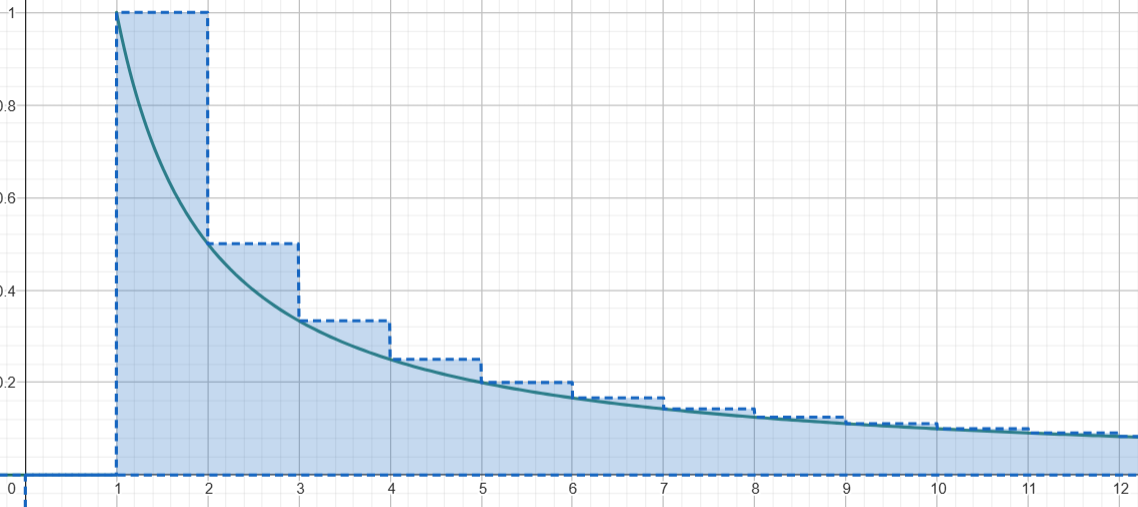
\includegraphics[width=36em]{Imagens/harmonicarea.png}

    E com esses resultados, sabemos que \(op(N,M) \geq C_1\times M \log N\) e \(op(N,M) \geq C_2\ \times N\), então, \(op(N,M)\geq \frac{1}{2}(C_1\times N + C_2 \times M \log N)\geq \frac{\min(C_1,C_2)}{2}(N+M \log N) \rightarrow \Omega(N+M \log N).\)

\newpage

\label{sol_c2.2.6}
\textbf{Solução do \hyperref[c2.2.6]{Exercício Adicional da Seção 2.2}}

Veja que a única possibilidade do valor de \(y\) diminuir é quando a seção \textbf{else} é executada, isto é, não houve nenhum \textbf{break} no código.

Para não haver nenhum break, todos os dez números \(x_i\) da lista \(x\) devem ter as seguintes propriedades:

\begin{enumerate}
    \item \(x_i \equiv 3\) (mod 5)
    \item \(x_i \equiv 4\) (mod 9)
    \item \(x_i \equiv 1\) (mod 11)
\end{enumerate}

Como queremos minimizar \(y\) e ele é definido como \(max_{i}(x_i)\), então no geral queremos encontrar os dez menores inteiros positivos que cumpram as três condições ao mesmo tempo.

Perceba que os módulos são primos entre si, portanto, esse problema cumpre as hipóteses do \href{https://en.wikipedia.org/wiki/Chinese_remainder_theorem}{Teorema Chinês dos Restos}, e portanto, podemos aplicar esse teorema, que possui uma boa explicação \href{https://www.youtube.com/watch?v=ru7mWZJlRQg}{neste vídeo}, do canal Math Made Easy.

Para achar o menor inteiro positivo que cumpre isso \(x_0\), faremos o seguinte:
\begin{itemize}
    \item \(x_0 = R_5 +R_9 + R_{11}\), onde \(R_5 \equiv 0\) (mod 9) e (mod 11), \(R_9 \equiv 0\) (mod 5) e (mod 11) e \(R_{11} \equiv 0\) (mod 5) e (mod 9).

    \item Para \(R_5\), precisamos que \(9 | R_5, 11 |R_5\) e \(R_5 \equiv 3\) (mod 5). Para encontrarmos isso, veja que queremos o menor múltiplo de \(99\) que possua resto \(3\) por \(5\), que podemos verificar rapidamente que é \(198\).

    \item Fazemos o análogo para \(R_{9}\), que nos exige o menor múltiplo de \(55\) com resto \(4\) por \(9\) que é \(220\) e também para \(R_{11}\), que nos exige o menor múltiplo de \(45\) com resto \(1\) por \(11\) que é o próprio \(45\).

    \item Portanto: \(x_0 = R_5+R_9+R_{11}=198+220+45=463\).
\end{itemize}

Agora que temos \(x_0\), basta ver que os próximos números devem ser obtidos na forma \(x_0+\alpha M\), onde \(M\) é o menor múltiplo positivo de 5, 9 e 11 ao mesmo tempo, que sabemos ser \(mmc(5,9,11)=495\).

Assim, os dez menores números que queremos são os números da forma \(463+495\alpha, \) com \(\alpha \in [0,9]\):

\begin{code}
x = [463 + 495 * k for k in range(10)]
\end{code}

\void[-1]

Aplicando esses valores para o vetor \(x\), podemos ver que o código será executado sem breaks, tornando \(y=463+9\times495=4918\).

\newpage

\label{sol_ex2.4.a}
\textbf{Solução do \hyperref[ex2.4.a]{Exercício Adicional da Seção 2.4}}

Note que nesse grafo, o grau de todo vértice é ao menos dois. Assim, dado um vértice \(u\), ele tem pelo menos um vizinho \(v\) e esse vizinho também tem outro vizinho \(w\) que não é vizinho de \(u\), já que o grafo não tem triângulos de vértices.

Porém, note que adicionar a aresta \(uw\) forma um triângulo de vértices. Assim, o grafo \(G+uw\) não pode ter seus vértices coloridos sem que vizinhos tenham a mesma cor justamente pela existência do triângulo.

Isso é verdade pois a restrição imposta nos força que \(cor(u) \ne cor(v)\), \(cor(u) \ne cor(w)\) e \(cor(v) \ne cor(w)\). Assim, seriam necessárias ao menos três cores para as três condições serem cumpridas ao mesmo tempo, o que não é o caso do nosso problema.

Grafos que possuem uma pintura descrita são chamados de \href{https://en.wikipedia.org/wiki/Bipartite_graph}{grafos bipartidos}, e é possível mostrar de forma simples que um grafo não é bipartido se e somente se ele possui um \textbf{ciclo ímpar}.

A ideia geral é ver que se considerarmos o algoritmo:

\begin{itemize}
    \item Pinte um nó inicial
    \item Pinte os vizinhos de todo nó pintado da cor oposta
\end{itemize}

Em um grafo e ele gerar algum conflito, então podemos concluir que existe uma sequência de vértices que formará um ciclo ímpar, direta ou indiretamente: siga a sequência dos vértices partindo dos dois que dão conflito e prosseguindo com quem pintou ele repetidamente até chegar a um vértice comum dos dois lados e verifique os possíveis casos.

Já para o outro lado, se existe um ciclo ímpar, então veja que é impossível termos uma pintura bem definida para o ciclo ímpar: basta reiterar o argumento descrito no caso do triângulo (pois um triângulo é um ciclo ímpar) e verá que existe um vértice que deve ter uma cor diferente tanto de azul quanto de vermelho.

\newpage

\label{sol_ex3.3.a}
\textbf{Solução do \hyperref[ex3.3.a]{Exercício Adicional da Seção 3.3}}

Esse é um exercício simples: basta se atentar ao código anterior e fazer modificações para que tudo fique dentro da classe. Segue uma possível solução esperada.

\begin{code}
class Heap:
    def __init__(self):
        self.h = ['max']
    
    def empty(self):
        return len(self.h) == 1
    
    def type(self):
        return self.h[0]
        
    def top(self):
        return self.h[1] if not self.empty() else None
    
    def push(self, x):
        nx = len(self.h)
        self.h.append(x)
        while(nx > 1):
            if self.h[nx] > self.h[nx//2]:
                self.h[nx],self.h[nx//2] = self.h[nx//2],self.h[nx]
                nx //= 2
            else:
                break
    
    def pop(self):
        if self.empty():
            return None
        nx = 1
        self.h[1], self.h[len(self.h)-1] = self.h[len(self.h)-1], self.h[1]
        while 2*nx <= len(self.h)-2:
            x = 0
            if 2*nx+1 > len(self.h)-2 or self.h[2*nx+1] < self.h[2*nx]:
                x = 2*nx
            else:
                x = 2*nx + 1
            if self.h[nx] < self.h[x]:
                self.h[x],self.h[nx] = self.h[nx],self.h[x]
                nx = x
            else:
                break
        return self.h.pop()

h = Heap()
h.push(3); h.push(8); h.push(5)
while not h.empty():
    print(h.pop())
\end{code}

\newpage

\label{sol_ex4.1.a}
\textbf{Solução do \hyperref[ex4.1.a]{Exercício Adicional da Seção 4.1}}

\begin{code}
import numpy as np
x = np.random.randint(low=100,high=1000001,size=10000,dtype='int32')

x1 = x[(x%16 == 0) & (x%32 != 0)]

x2 = x[(x%9 == 0)]

x3 = x[np.floor(x**0.5)**2 == x]

x4 = x[((x^(x-1))+1) == 2*x]

x5 = x[(x%7 == 0)&(((x//7)^(x//7 - 1))+1 == 2*(x//7))]

x6 = x[(((x^(x-1))+1)/2)*(((x^(x-1))+3)/2) == x]

x7 = x[((x&(~31))%3 == 0) & ((((x&(~31))//3)&(-((x&(~31))//3)))==((x&(~31))//3)) & (3*(2**(x-(x&(~31)))) == (x&(~31)))]
\end{code}

\begin{enumerate}
    \item Basta verificar as condições de multiplicidade naturalmente usando a notação de indexação booleana.

    \item Veja que a soma dos dígitos ser um múltiplo de 9 é um critério de divisibilidade por 9, portanto, basta encontrar os múltiplos de 9.

    \item Se um número é quadrado perfeito, ele tem raiz quadrada exata. Assim, basta elevarmos o piso da raiz quadrada ao quadrado e verificar se isso é o número original, pois se o número não for quadrado perfeito, esse valor vai ser menor.

    \item Podemos calcular a menor potência de 2 na representação binária do número e comparar com ele mesmo. Para isso, podemos usar a mesma identidade do exercício da seção 1.2 ou ainda a seguinte: \((x\&(-x)) == x\), pois pela forma que os números negativos são armazenados binariamente, o único bit igual a 1 é o bit da menor potência de 2 do número.

    \item Se um número for dessa forma, então ele tanto é múltiplo de 7 quanto o número \(x/7\) é uma potência de 2, então basta verificar essas duas condições usando coisas que vimos nos itens anteriores.

    \item Se um número é dessa forma, então podemos encontrar a menor potência de 2 que existe nele, multiplicar pelo sucessor dela e isso deve ser o valor do número original.

    \item Veja que se um número é daquela forma nos intervalos do problema, então \(k<20\), pois \(2^{20}>1000000\). Com isso, veja que se apagarmos os últimos 5 dígitos binários de \(x\) usando \(y=(x \&\) \til \(31)\) (operador e-lógico na negação de 31), devemos ter um número da forma \(3\times 2^k\). Com isso garantido, basta verificar se \(3\times2^{x-y}+(x-y)=x\), isto é, \(3\times2^{x-y}=y\). 
\end{enumerate}

\newpage

\label{sol_ex5.2.a}
\textbf{Solução do \hyperref[ex5.2.a]{Exercício Adicional da Seção 5.2}}

Veja que o código \textbf{findeps} dado no documento faz: dado um valor \(y\) e número de iterações, encontra o épsilon de máquina ao redor de \(y\). Nosso problema aqui é um pouco diferente: não sabemos o \(y\), mas sabemos o \(\emaq\).

Há várias formas de fazer esse problema, mas uma bem simples é basicamente reaplicar uma busca binária: comece com os limites entre 0 e o \textbf{float máximo} e aplique uma busca binária para verificar se o épsilon de máquina está maior ou menor que \(x\). 

Pela natureza dos números de ponto flutuante, se o número aumenta o épsilon de máquina também, e se o número diminui, o mesmo acontece (observação: em módulo, pois números negativos são equivalentes aos positivos nesse contexto), o que faz a busca binária funcionar.

Assim, implementamos essa ideia com uma pequena variação: fazemos o nosso critério de parada ser algum dos extremos do intervalo não alterar em uma iteração ao invés de um número fixo de iterações, e também importamos a função findeps usada no documento a critério de validade da nossa resposta.

\begin{code}
from documento import findeps
import sys

def adapteps(x):
    left = 0; right = sys.float_info.max; previous = 1
    while right != previous and left != previous:
        mid = (left + right)/2
        inf = 0; sup = mid; prev = mid+1
        while prev != sup and prev != inf:
            eps = (inf + sup)/2
            if (mid + eps == mid):
                prev = inf
                inf = eps
            else:
                prev = sup
                sup = eps
        if 2*sup > x:
            previous = right
            right = mid
        else:
            previous = left
            left = mid
    return left

x = -100
print(f'O épsilon de máquina para {adapteps(2**x):.2e} é {findeps(adapteps(2**x),10000):.2e}. Valor esperado: {2**x:.2e}.')
\end{code}

Veja que a resposta foi dada como \textbf{.2e}, que é a notação para representar floats em notação científica com duas casas decimais de precisão.

\end{document}